\chapter{Violation in Crossover Distribution} \label{ch:chiviolation}
This chapter explores the robustness of finite population oscillation when condition \ref{OscCond} 
for the crossover distribution is violated and infinite population trajectories
have no periodic orbit.

Error $\bm{\epsilon}$ is introduced into the crossover distribution $\bm{\chi}$ so as to 
violate condition \ref{OscCond}; this guarantees that 
infinite population trajectories have no periodic orbit. Consequently, $\bm{p}^\ast \;=\; \bm{q}^\ast \;=\; \bm{z}^\ast$. 
Violation of the condition \ref{OscCond} for $\bm{\chi}$, crossover-violation,  
can numerically be expressed as:\newline  
for all $g$,  $g \neq 0$,
\begin{equation}
\label{chi-violation}
  1 \neq \sum \limits_{k \in \bar{g}\mathcal{R}} \bm{\chi}_{k+g} + \bm{\chi}_k  
\end{equation}

Going forward, we use `limit $\bm{z}^\ast$' to denote evolutionary limit when crossover distribution 
$\bm{\chi}$ violates condition \ref{OscCond}, and 
`non-violation limits $\bm{p}^\ast$ and $\bm{q}^\ast$' to denote limits without violations (i.e., $\bm{\epsilon \,=\, 0}$).

\section{Violation}
The crossover distribution $\bm{\chi}$ was modified as
\[
\bm{\chi}_i = (1-\bm{\epsilon}) \bm{\chi}_i\ 
\]
So that 
\[
\bm{\chi}_i + \bm{\chi}_{i+g} = 1-\bm{\epsilon} ; \tabspace g \text{ is defined in  section } \ref{Limits}
\]
Then a single $j$ is chosen where $j \not\in \bar{g}\mathcal{R}$ and we set $\bm{\chi}_j = \bm{\epsilon}$. 

Violation in crossover distribution $\bm{\chi}$ is different from violation in mutation distribution $\bm{\mu}$. 
The Markov chain formed by transition matrix $Q$ is regular under violation in $\bm{\mu}$ 
but that need not be the case under violation in  $\bm{\chi}$. 
% With $\bm{\chi}$ described above, non-crossover mask (all 0s) has always positive probability. 
% And since we do not modify the mutation distribution $\bm{\mu}$ satisfying condition \ref{OscCond}, 
% the non-mutation mask (all 0s) has always zero probability. 
% However, applying same mutation mask twice with non-crossover event, 
% we can achieve non mutation event in two generations. 
% 
% % Let us exlore for two cases of $g$ in \ref{OscCond}:
% % 
% % 1. When $g$ is all $1$s:\newline
% % Any mask with a $1$ at position $k$ ($0 \leq k < \ell$) and $0$ at all other positions can mutate the $k$th bit of a string.  In next step, 
% % either the string can mutate its next bit or the string can simulate non-mutation event in two generations (mutate $j$th bit twice). 
% % This makes possibile for any string to mutate to 
% % any other string. And any string can maintain its bits in even number of generations after aquiring its state. 
% % 
% % 2. When $g$ has atleast one $0$:\newline
% % Any mask with a $1$ at position $k$ and $0$ at all other positions  
% % will have positive probability if $g$ also is $1$ at position $k$. 
% % Thus any bit where $g$ is $1$ can mutate.  
% % Any mask with $1$ in just one of the positions where $g$ has $1$s and 
% % also $1$ in just one of the positions where $g$ has $0$s can be used to 
% % mutate a bit where $g$ is $0$ using two masks in sequence. 
% % So any string can mutate to any other. 
% % Also any string requires two generations to simulate non-mutation event. 
% 
% Any mask with a $1$ at position $k$ and $0$ at all other positions  
% will have positive probability if $g$ also is $1$ at position $k$. 
% Thus any bit where $g$ is $1$ can mutate. 
% 
% 1. Mutate a bit in string where $g$ has $0$: 
% Any mask with $1$ in just one of the positions where $g$ has $1$s and 
% also $1$ in just one of the positions where $g$ has $0$s can be used to 
% mutate a bit where $g$ is $0$ using these two masks in sequence in two steps. 
% 
% 2.
% Any bit in a string at position where $g$ 
% is $1$ can be mutated in two steps. 
% 
% So any string can mutate to any other in even number of steps. 
% Also any string requires two generations to simulate non-mutation event.
% So any population can therefore mutate to any other population in even number of generations, 
% and that makes the Markov chain irreducible.
% 
% In this research, experiment is designed to have finite population size as multiple of 2. 
% So, there is a special set of population $P_s$ which can mutate to itself, i.e. one string in 
% population can mutate to another string in population maintaining same population member strings within. 
% Since any population can mutate to any other population, let us assume finite population $P_i$ 
% can reach special population $P_s$ in $u$ (even) generations. Population $P_s$ can stay in its state as long as its wants 
% by mutating to itself or mutate to next population state. Population $P_s$ can return to $P_i$ next $u$ generations. 
% Let's say $P_s$ stays as $P_s$ for $h$ generations. Then population $P_i$ can return to its original state $P_i$ 
% in total $2u+h$ generations. $h$ can be $1, \; 2, \;, 3,$ and so on. That means $P_i$ can return to its original state in 
% odd or even number of generations. So, the Markov chain is also aperiodic.
% 
% Since the Markov chain formed by GA after the violation in $\bm{\chi}$ is irreducible and aperiodic, 
% the Markov chain is regular (see \cite{Iosifescu1980}), and a steady state distribution 
% with positive components exists for the GA (see \cite{Minc1988}). 
The initial population is 
computed using the same procedure as described in section \ref{InitPopOsc}. To explore the effects of the degree  
of violation of condition \ref{OscCond} in $\bm{\chi}$, different values of $\bm{\epsilon} \in \{0.01, 0.1, 0.5\} $ are used in experiments. 
String length $\ell \;\in\; \{8, 10, 12, 14\}$ is considered for simulation.
The distances of both infinite and finite populations to limit $\bm{z}^\ast$ are plotted. 
The distances of both infinite and finite populations to non-violation limits $\bm{p}^\ast$ and $\bm{q}^\ast$ are also plotted.

\clearpage
% figures for chi violation
\subsection{Haploid Population $\mathtt{\sim}$ $\epsilon: 0.01$}

% l = 8
\begin{figure}[h]
\begin{center}
\subfloat{
\resizebox{8cm}{5cm}{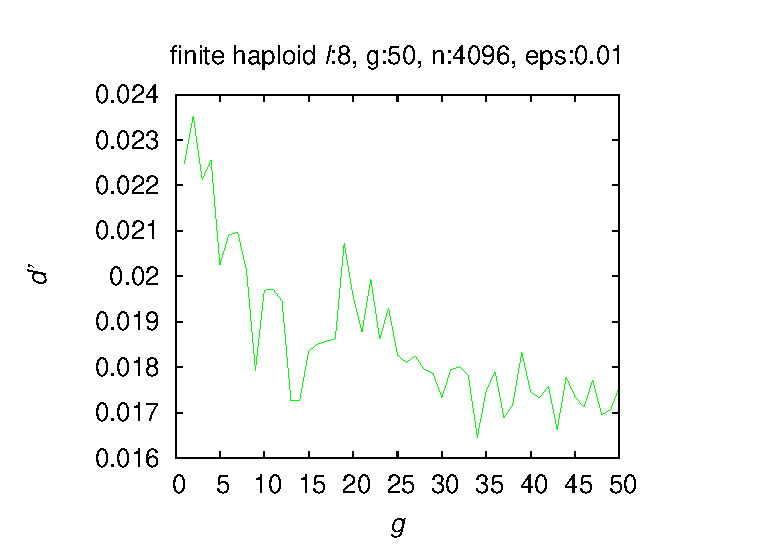
\includegraphics{figures/eps/vio/chi/b8/e0.01/n00004096_fin_hap.eps}}} \hspace{-3em}%
\subfloat{
\resizebox{8cm}{5cm}{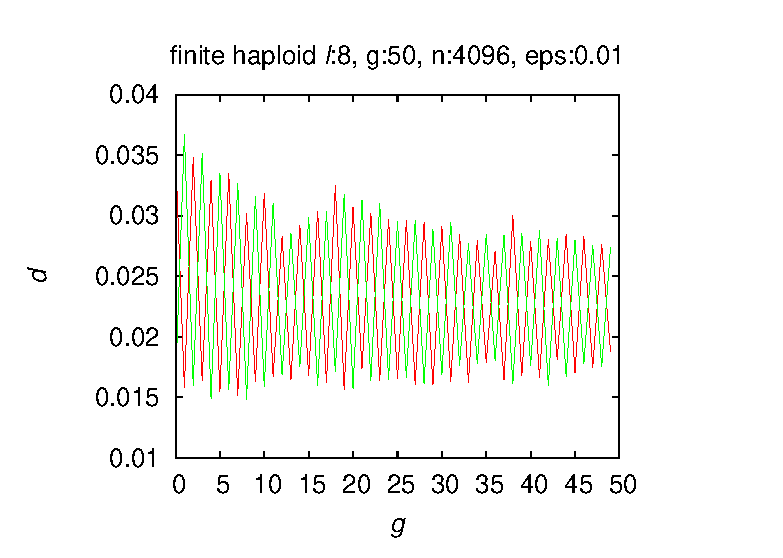
\includegraphics{figures/eps/vio/chi/b8/e0.01/n00004096_fin_hap_wovio.eps}}}\vspace{-1em} \hspace{-3em}%
\end{center}
\begin{center}
\subfloat{
\resizebox{8cm}{5cm}{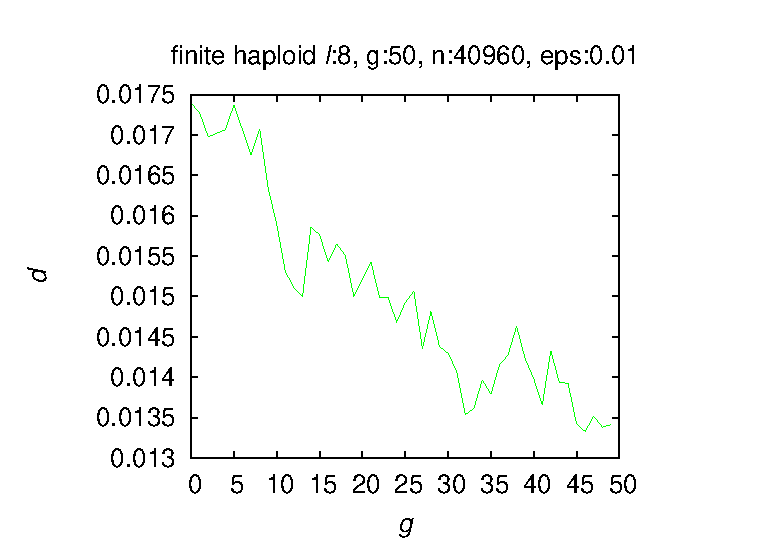
\includegraphics{figures/eps/vio/chi/b8/e0.01/n00040960_fin_hap.eps}}} \hspace{-3em}%
\subfloat{
\resizebox{8cm}{5cm}{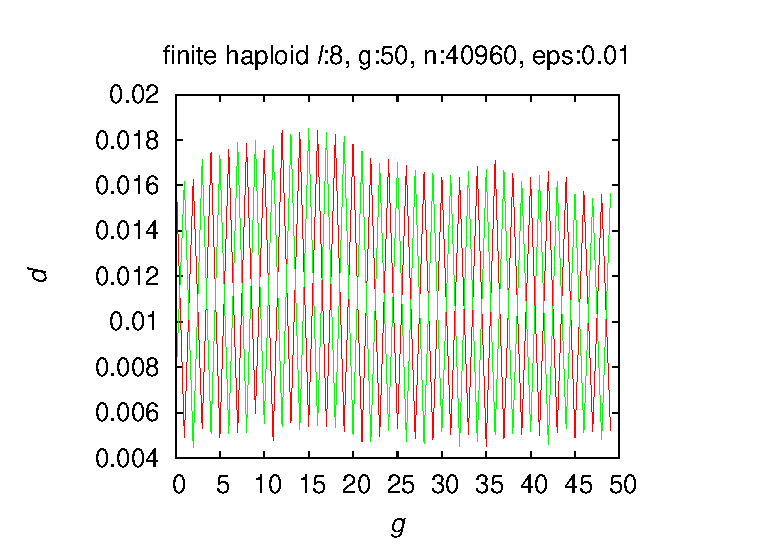
\includegraphics{figures/eps/vio/chi/b8/e0.01/n00040960_fin_hap_wovio.eps}}}\vspace{-1em} \hspace{-3em}%
\end{center}
\end{figure}

\begin{figure}[h]

\begin{center}
\subfloat{
\resizebox{8cm}{5cm}{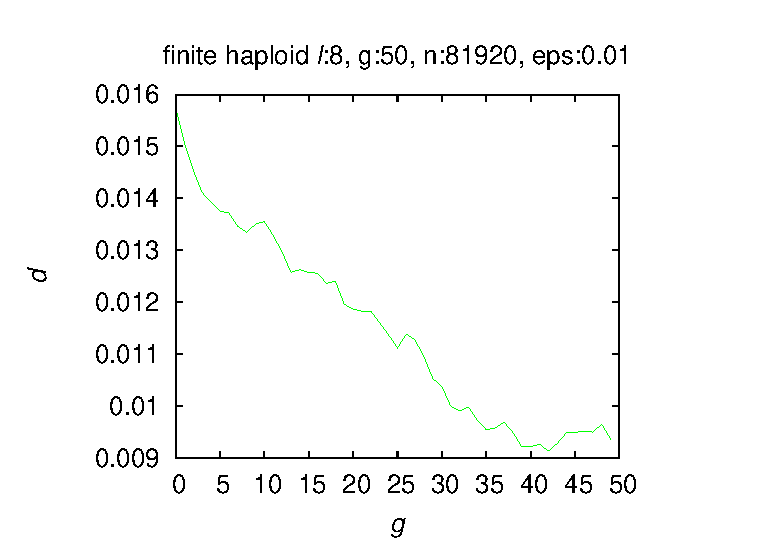
\includegraphics{figures/eps/vio/chi/b8/e0.01/n00081920_fin_hap.eps}}} \hspace{-3em}%
\subfloat{
\resizebox{8cm}{5cm}{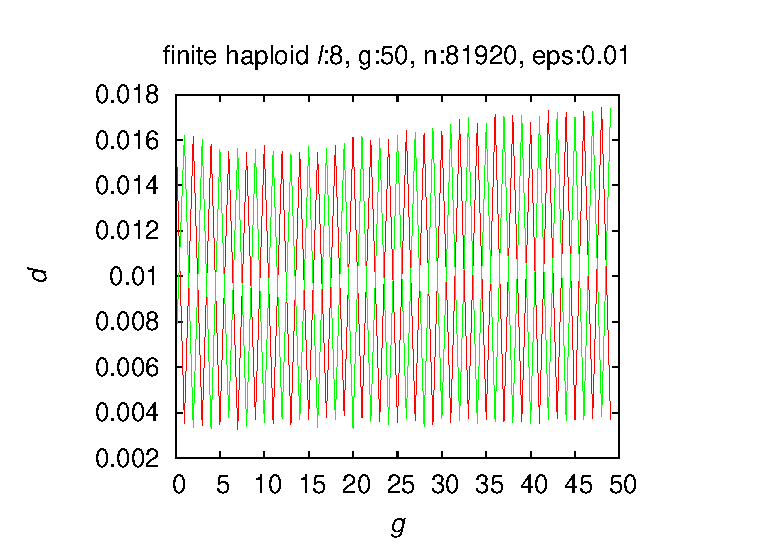
\includegraphics{figures/eps/vio/chi/b8/e0.01/n00081920_fin_hap_wovio.eps}}}\vspace{-1em} \hspace{-3em}%
\end{center}

\begin{center}
\subfloat{
\resizebox{8cm}{5cm}{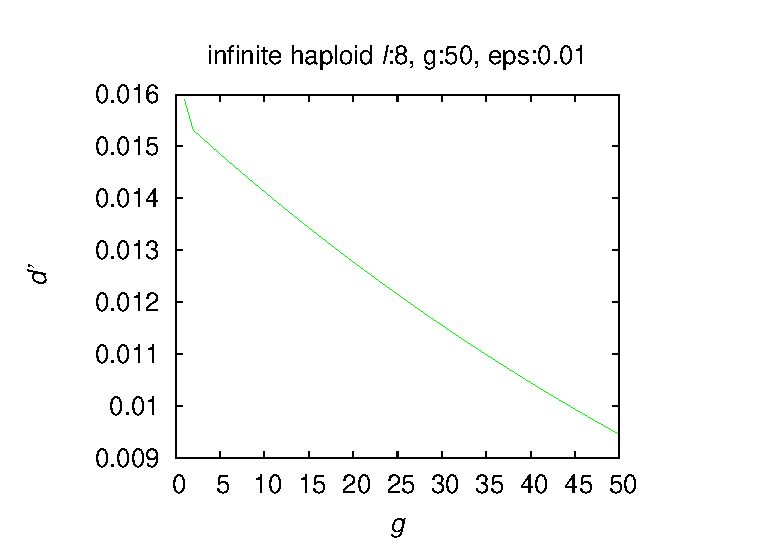
\includegraphics{figures/eps/vio/chi/b8/e0.01/inf_hap.eps}}}\hspace{-3em}%
\subfloat{
\resizebox{8cm}{5cm}{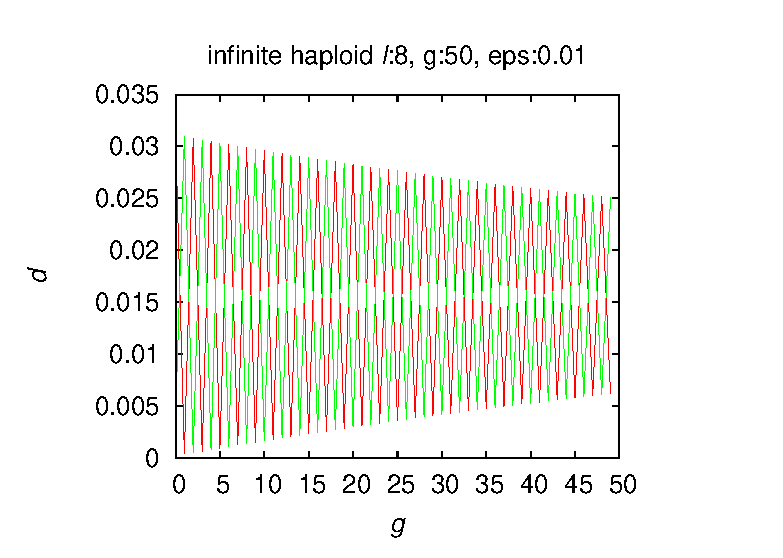
\includegraphics{figures/eps/vio/chi/b8/e0.01/inf_hap_wovio.eps}}}\vspace{-0.5em} \hspace{-3em}%


\caption[\textbf{Infinite and finite haploid population oscillation behavior in case of violation in $\bm{\chi}$ for genome length $\ell = 8$ and $\bm{\epsilon} = 0.01$}]{\textbf{Infinite and finite haploid population oscillation behavior in case of violation in $\bm{\chi}$ for genome length $\ell = 8$ and $\bm{\epsilon} = 0.01$:} 
  In left column, $d'$ is distance of finite population of size $n$ or infinite population to limit $\bm{z}^\ast$ for $g$ generations. In right column, $d$ is distance of finite population or infinite population to limits $\bm{p}^\ast$ and $\bm{q}^\ast$ without violation.}
\label{oscillation_8h_vio_chi_0.01}
\end{center}
\end{figure}


% l = 10

\begin{figure}[h]
\begin{center}
\subfloat{
\resizebox{8cm}{5cm}{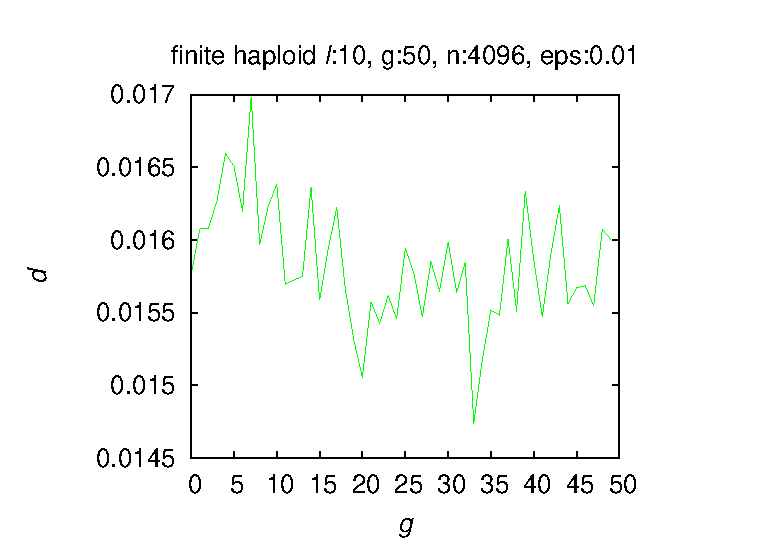
\includegraphics{figures/eps/vio/chi/b10/e0.01/n00004096_fin_hap.eps}}} \hspace{-3em}%
\subfloat{
\resizebox{8cm}{5cm}{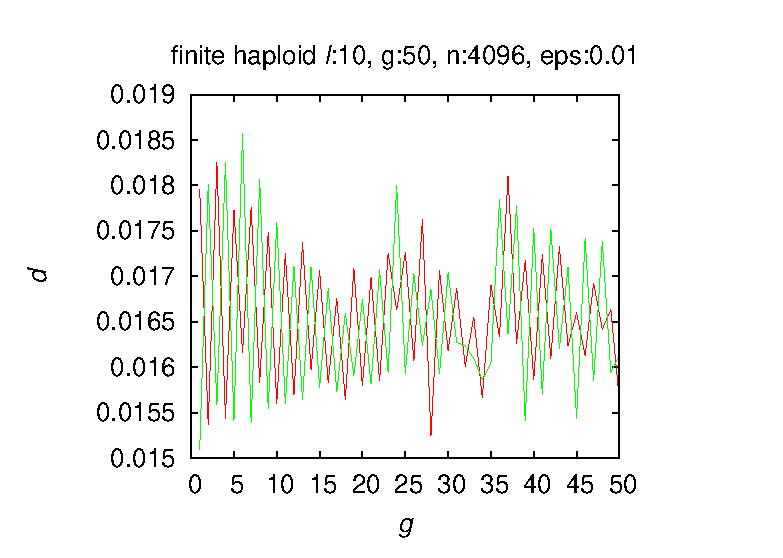
\includegraphics{figures/eps/vio/chi/b10/e0.01/n00004096_fin_hap_wovio.eps}}}\vspace{-1em} \hspace{-3em}%
\end{center}
\begin{center}
\subfloat{
\resizebox{8cm}{5cm}{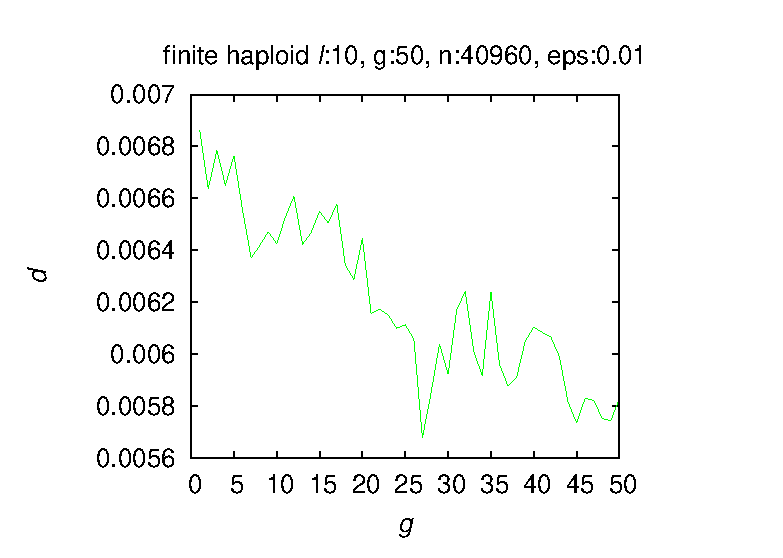
\includegraphics{figures/eps/vio/chi/b10/e0.01/n00040960_fin_hap.eps}}} \hspace{-3em}%
\subfloat{
\resizebox{8cm}{5cm}{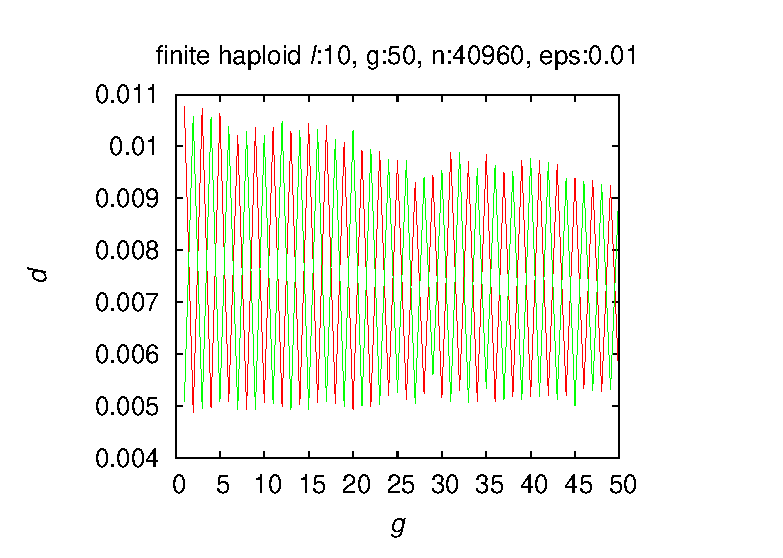
\includegraphics{figures/eps/vio/chi/b10/e0.01/n00040960_fin_hap_wovio.eps}}}\vspace{-1em} \hspace{-3em}%
\end{center}

\begin{center}
\subfloat{
\resizebox{8cm}{5cm}{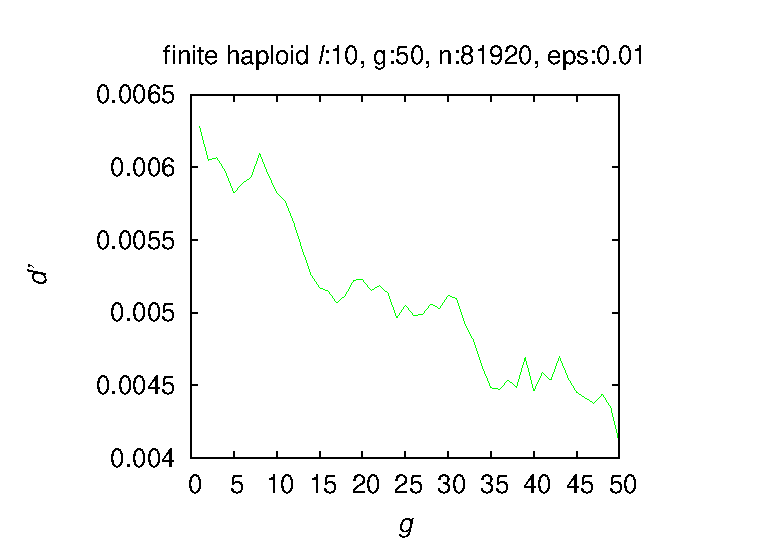
\includegraphics{figures/eps/vio/chi/b10/e0.01/n00081920_fin_hap.eps}}} \hspace{-3em}%
\subfloat{
\resizebox{8cm}{5cm}{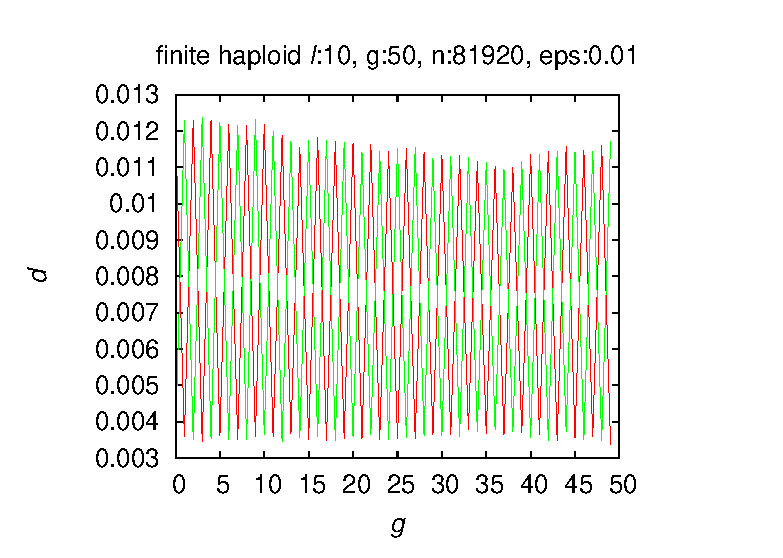
\includegraphics{figures/eps/vio/chi/b10/e0.01/n00081920_fin_hap_wovio.eps}}}\vspace{-1em} \hspace{-3em}%
\end{center}

\begin{center}
\subfloat{
\resizebox{8cm}{5cm}{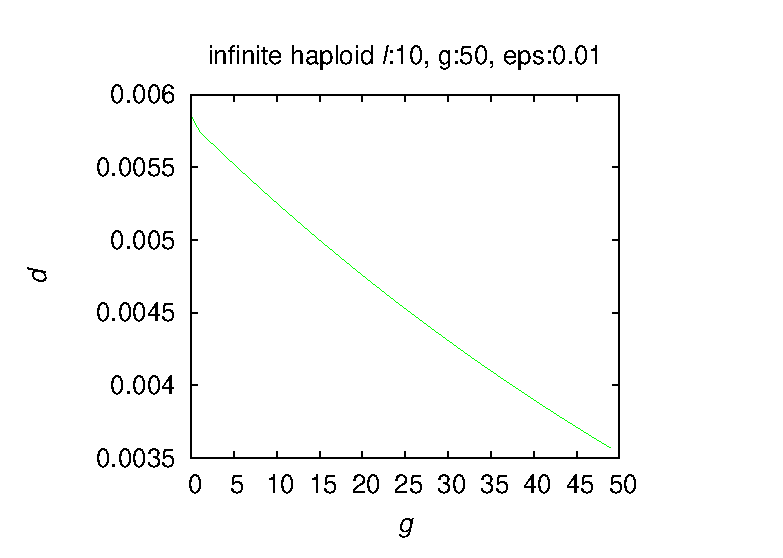
\includegraphics{figures/eps/vio/chi/b10/e0.01/inf_hap.eps}}}\hspace{-3em}%
\subfloat{
\resizebox{8cm}{5cm}{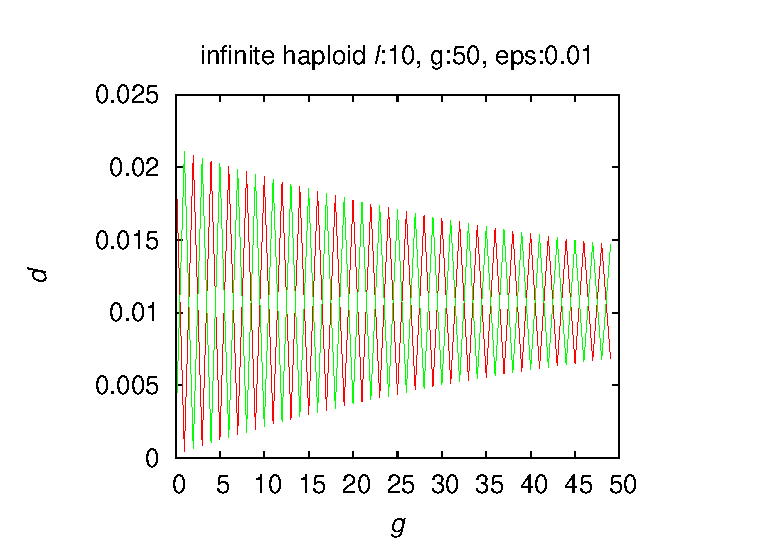
\includegraphics{figures/eps/vio/chi/b10/e0.01/inf_hap_wovio.eps}}}\vspace{-0.5em} \hspace{-3em}%

\caption[\textbf{Infinite and finite haploid population oscillation behavior in case of violation in $\bm{\chi}$ for genome length $\ell = 10$ and $\bm{\epsilon} = 0.01$}]{\textbf{Infinite and finite haploid population oscillation behavior in case of violation in $\bm{\chi}$ for genome length $\ell = 10$ and $\bm{\epsilon} = 0.01$:} 
  In left column, $d'$ is distance of finite population of size $n$ or infinite population to limit $\bm{z}^\ast$ for $g$ generations. In right column, $d$ is distance of finite population or infinite population to limits $\bm{p}^\ast$ and $\bm{q}^\ast$ without violation.}
\label{oscillation_10h_vio_chi_0.01}
\end{center}
\end{figure}


% l = 12
\begin{figure}[h]
\begin{center}
\subfloat{
\resizebox{8cm}{5cm}{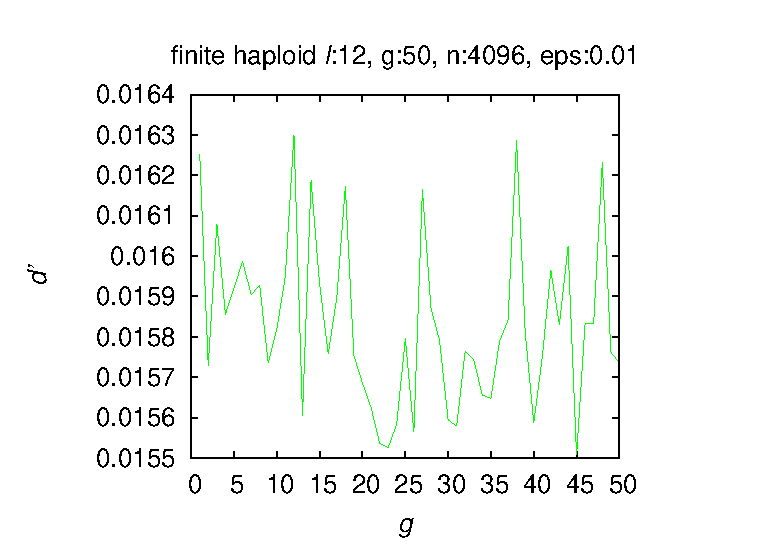
\includegraphics{figures/eps/vio/chi/b12/e0.01/n00004096_fin_hap.eps}}} \hspace{-3em}%
\subfloat{
\resizebox{8cm}{5cm}{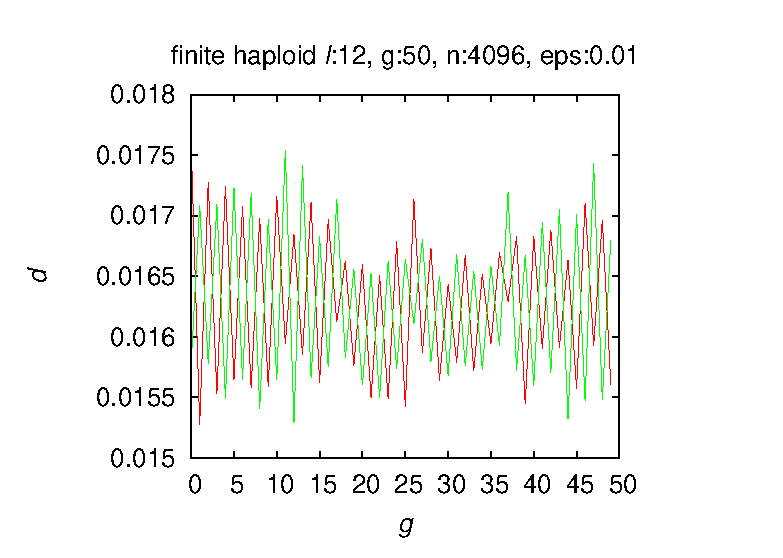
\includegraphics{figures/eps/vio/chi/b12/e0.01/n00004096_fin_hap_wovio.eps}}}\vspace{-1em} \hspace{-3em}%
\end{center}
\begin{center}
\subfloat{
\resizebox{8cm}{5cm}{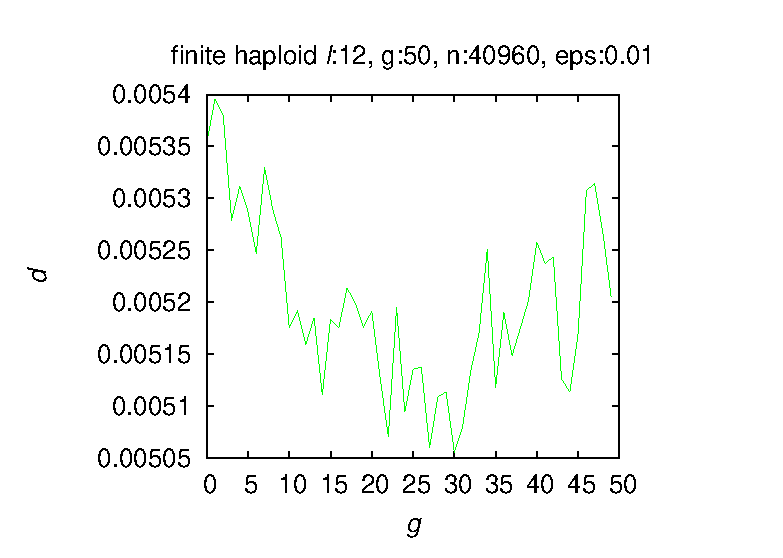
\includegraphics{figures/eps/vio/chi/b12/e0.01/n00040960_fin_hap.eps}}} \hspace{-3em}%
\subfloat{
\resizebox{8cm}{5cm}{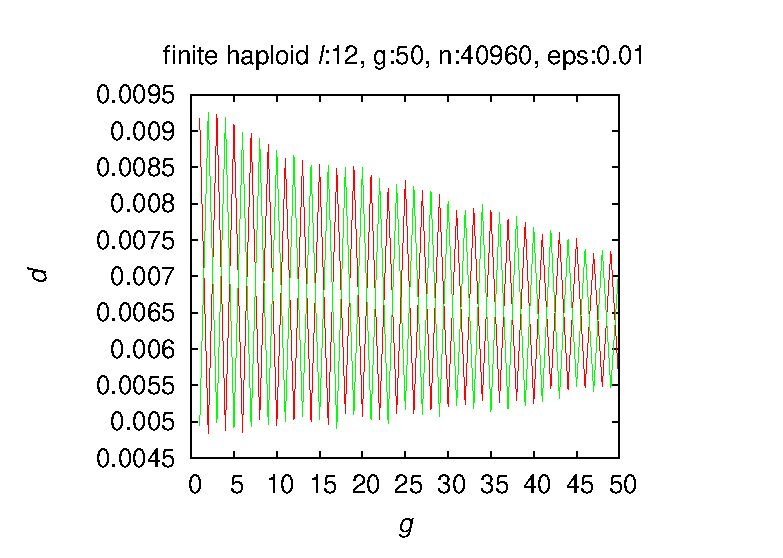
\includegraphics{figures/eps/vio/chi/b12/e0.01/n00040960_fin_hap_wovio.eps}}}\vspace{-1em} \hspace{-3em}%
\end{center}

\begin{center}
\subfloat{
\resizebox{8cm}{5cm}{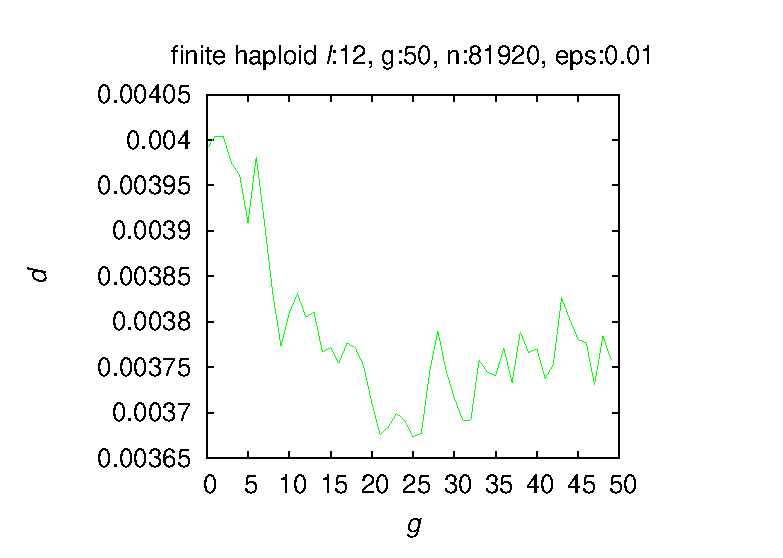
\includegraphics{figures/eps/vio/chi/b12/e0.01/n00081920_fin_hap.eps}}} \hspace{-3em}%
\subfloat{
\resizebox{8cm}{5cm}{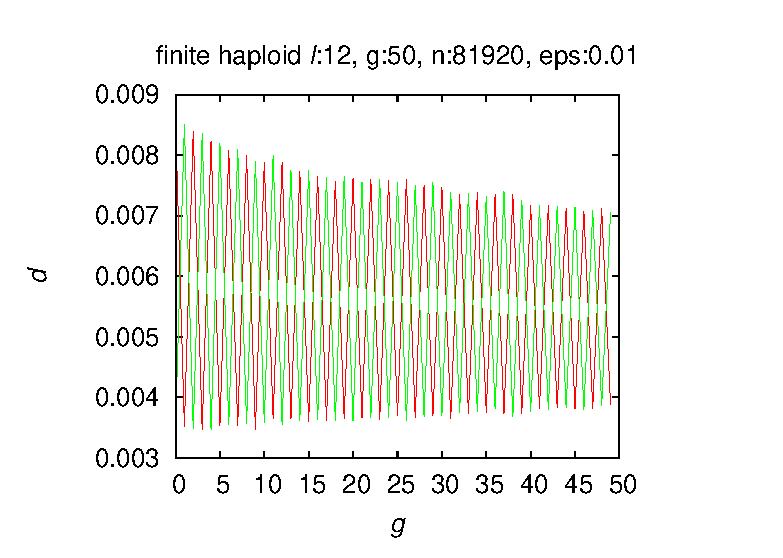
\includegraphics{figures/eps/vio/chi/b12/e0.01/n00081920_fin_hap_wovio.eps}}}\vspace{-1em} \hspace{-3em}%
\end{center}

\begin{center}
\subfloat{
\resizebox{8cm}{5cm}{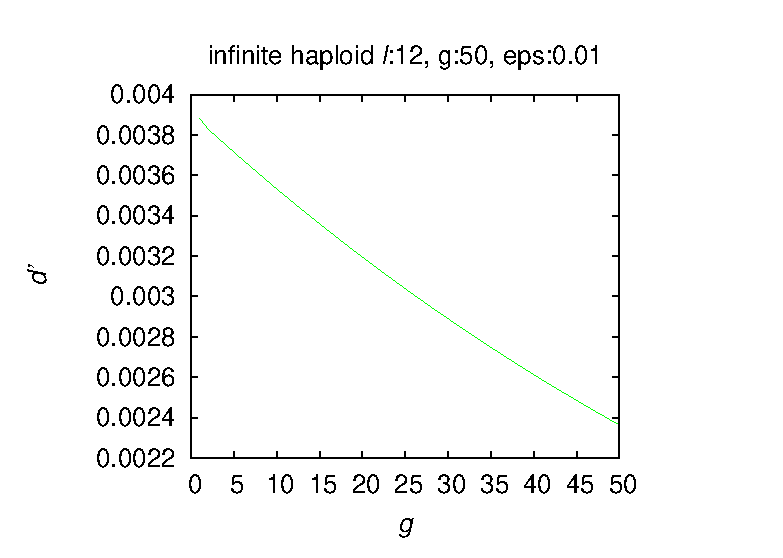
\includegraphics{figures/eps/vio/chi/b12/e0.01/inf_hap.eps}}}\hspace{-3em}%
\subfloat{
\resizebox{8cm}{5cm}{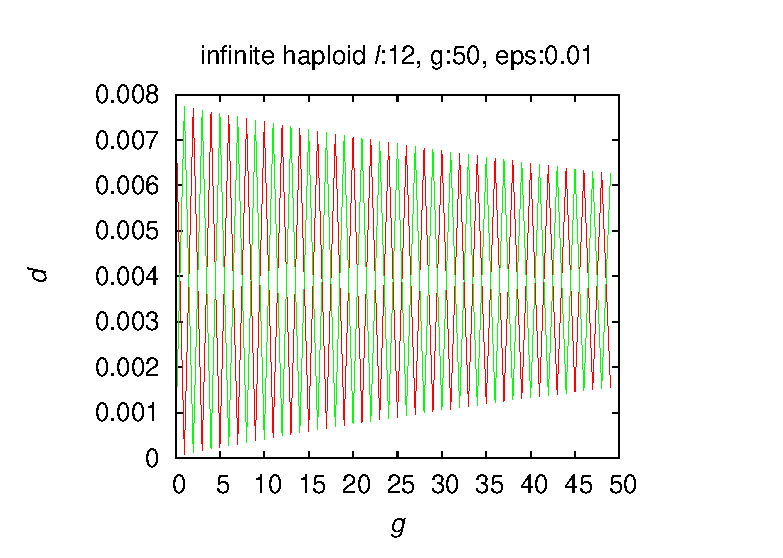
\includegraphics{figures/eps/vio/chi/b12/e0.01/inf_hap_wovio.eps}}}\vspace{-0.5em} \hspace{-3em}%


\caption[\textbf{Infinite and finite haploid population oscillation behavior in case of violation in $\bm{\chi}$ for genome length $\ell = 12$ and $\bm{\epsilon} = 0.01$}]{\textbf{Infinite and finite haploid population oscillation behavior in case of violation in $\bm{\chi}$ for genome length $\ell = 12$ and $\bm{\epsilon} = 0.01$:} 
  In left column, $d'$ is distance of finite population of size $n$ or infinite population to limit $\bm{z}^\ast$ for $g$ generations. In right column, $d$ is distance of finite population or infinite population to limits $\bm{p}^\ast$ and $\bm{q}^\ast$ without violation.}
\label{oscillation_12h_vio_chi_0.01}
\end{center}
\end{figure}

% l = 14

\begin{figure}[h]
\begin{center}
\subfloat{
\resizebox{8cm}{5cm}{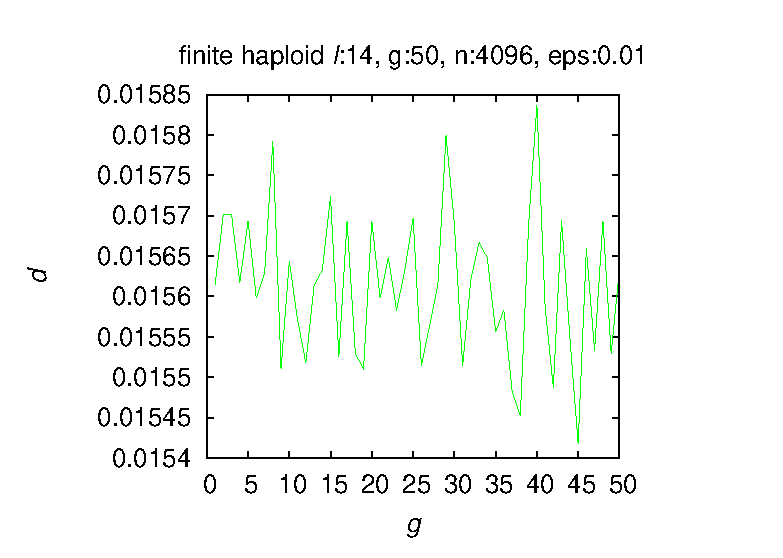
\includegraphics{figures/eps/vio/chi/b14/e0.01/n00004096_fin_hap.eps}}} \hspace{-3em}%
\subfloat{
\resizebox{8cm}{5cm}{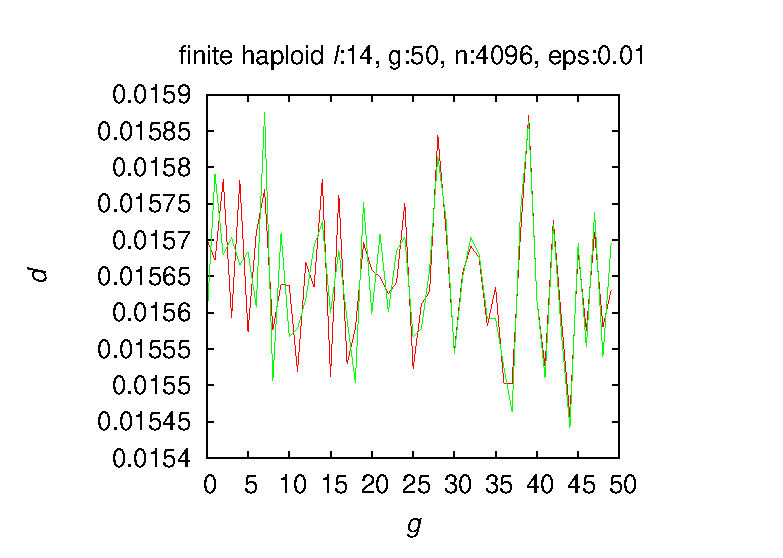
\includegraphics{figures/eps/vio/chi/b14/e0.01/n00004096_fin_hap_wovio.eps}}}\vspace{-1em} \hspace{-3em}%
\end{center}
\begin{center}
\subfloat{
\resizebox{8cm}{5cm}{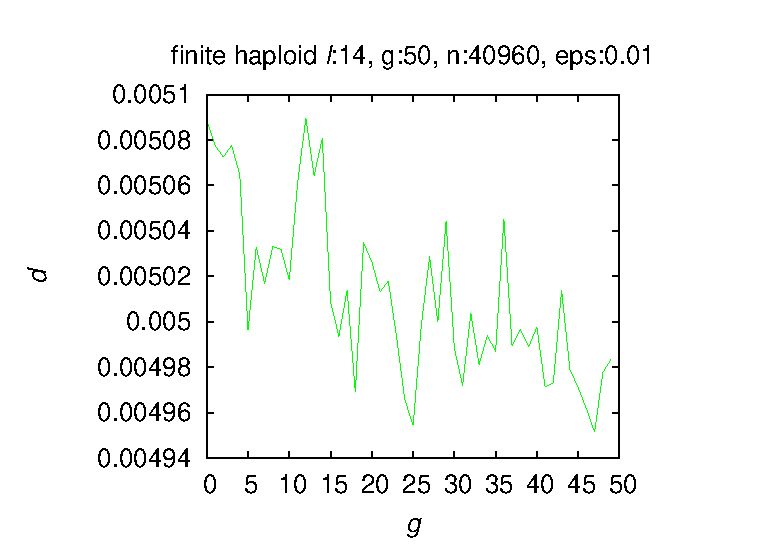
\includegraphics{figures/eps/vio/chi/b14/e0.01/n00040960_fin_hap.eps}}} \hspace{-3em}%
\subfloat{
\resizebox{8cm}{5cm}{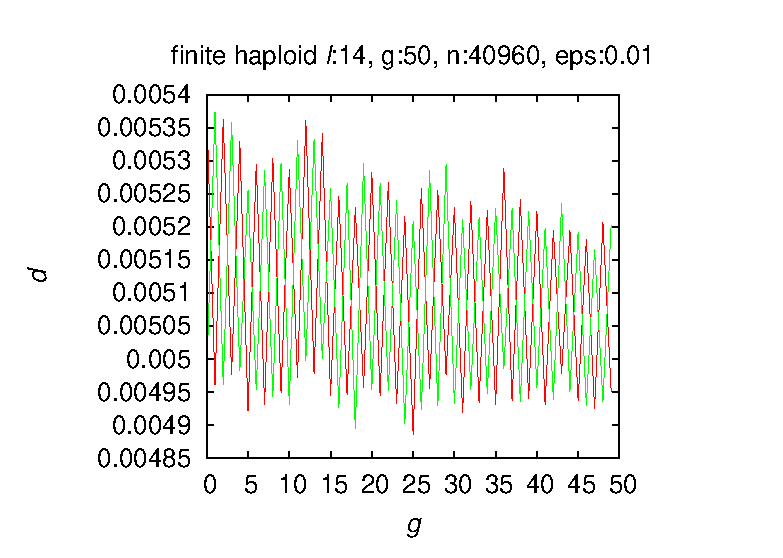
\includegraphics{figures/eps/vio/chi/b14/e0.01/n00040960_fin_hap_wovio.eps}}}\vspace{-1em} \hspace{-3em}%
\end{center}

\begin{center}
\subfloat{
\resizebox{8cm}{5cm}{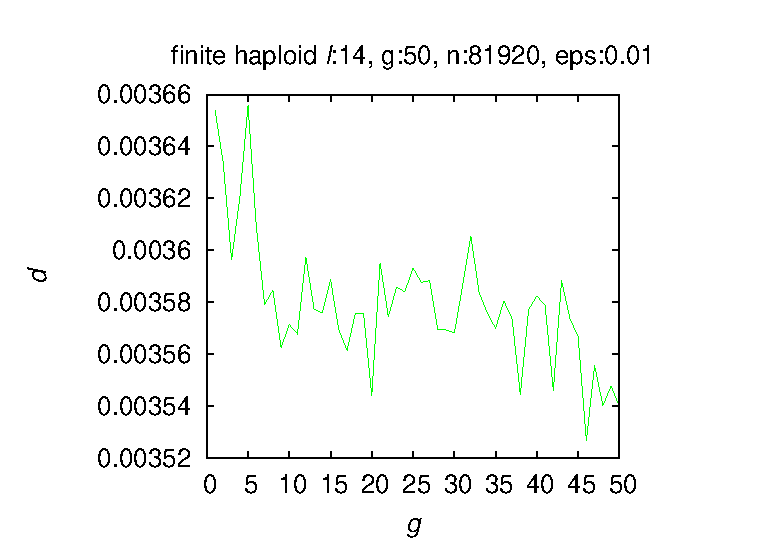
\includegraphics{figures/eps/vio/chi/b14/e0.01/n00081920_fin_hap.eps}}} \hspace{-3em}%
\subfloat{
\resizebox{8cm}{5cm}{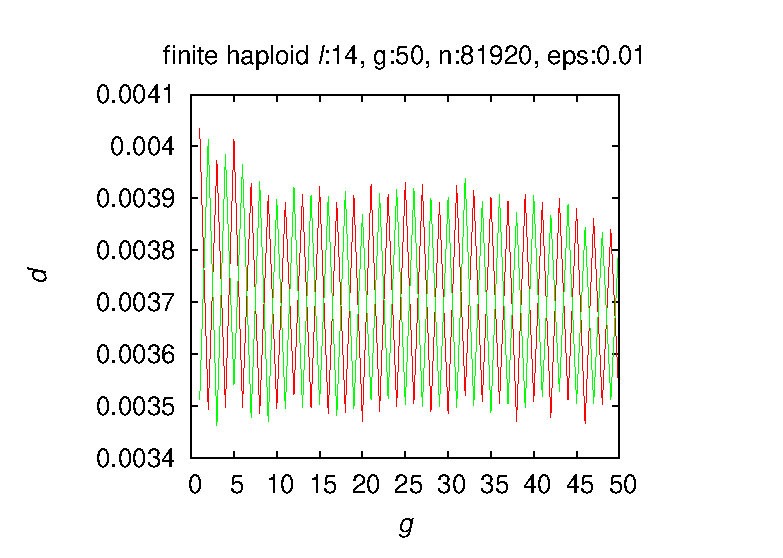
\includegraphics{figures/eps/vio/chi/b14/e0.01/n00081920_fin_hap_wovio.eps}}}\vspace{-1em} \hspace{-3em}%
\end{center}

\begin{center}
\subfloat{
\resizebox{8cm}{5cm}{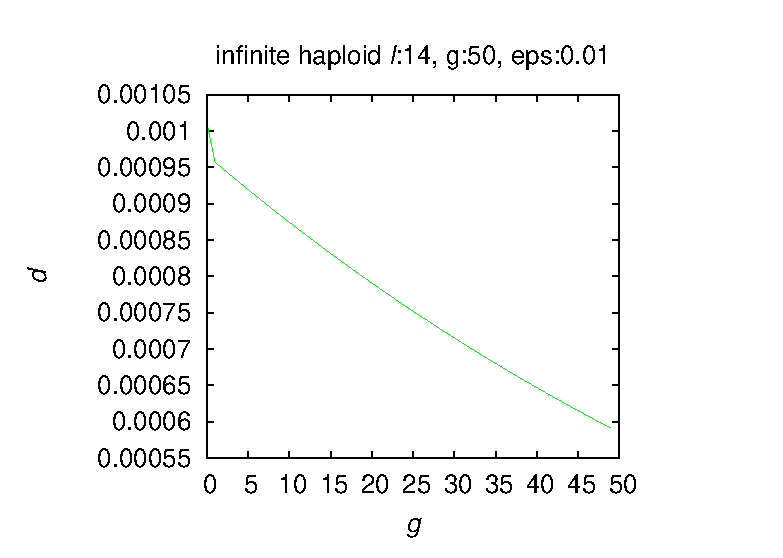
\includegraphics{figures/eps/vio/chi/b14/e0.01/inf_hap.eps}}}\hspace{-3em}%
\subfloat{
\resizebox{8cm}{5cm}{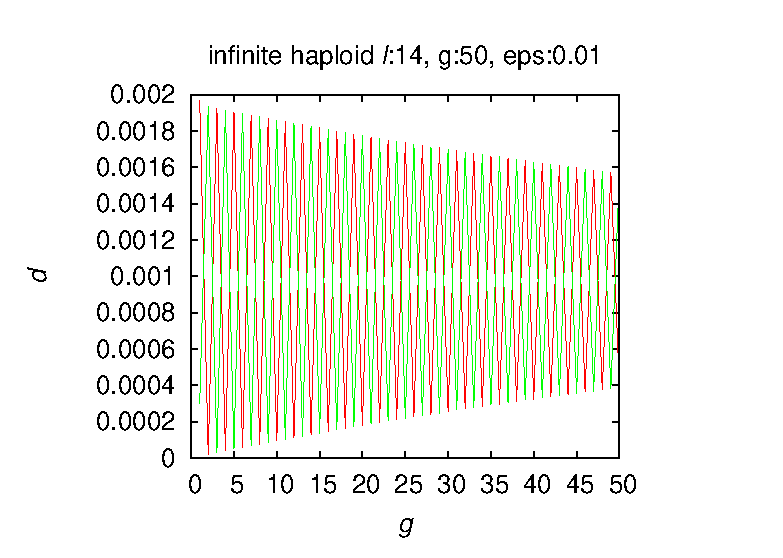
\includegraphics{figures/eps/vio/chi/b14/e0.01/inf_hap_wovio.eps}}}\vspace{-0.5em} \hspace{-3em}%

\caption[\textbf{Infinite and finite haploid population oscillation behavior in case of violation in $\bm{\chi}$ for genome length $\ell = 14$ and $\bm{\epsilon} = 0.01$}]{\textbf{Infinite and finite haploid population oscillation behavior in case of violation in $\bm{\chi}$ for genome length $\ell = 14$ and $\bm{\epsilon} = 0.01$:} 
  In left column, $d'$ is distance of finite population of size $n$ or infinite population to limit $\bm{z}^\ast$ for $g$ generations. In right column, $d$ is distance of finite population or infinite population to limits $\bm{p}^\ast$ and $\bm{q}^\ast$ without violation.}
\label{oscillation_14h_vio_chi_0.01}
\end{center}
\end{figure}

\clearpage

The right column in figures \ref{oscillation_8h_vio_chi_0.01} through \ref{oscillation_14h_vio_chi_0.01} 
shows distance of finite and infinite haploid populations to non-violation limits $\bm{p^\ast}$ and $\bm{q^\ast}$ with $\bm{\epsilon} \;=\; 0.01$. 
Those graphs indicate oscillating behavior of haploid populations given violation. 
Both finite and infinite populations oscillate given violation. Since the value of $\bm{\epsilon}$ 
is small, damping of ripples is slow. A new mask with positive probability created in crossover distribution with $\bm{\epsilon} \;=\; 0.01$ has small 
probability of being used during crossover and when they are not used, behavior should be consistent with 
the behavior without violation in the distribution. Moreover, $\bm{\epsilon} \;=\; 0.01$ is so small that 
infinite population oscillation does not die out in 50 generations but will die out eventually as generation progresses. 

The left column of figures \ref{oscillation_8h_vio_chi_0.01} through \ref{oscillation_14h_vio_chi_0.01} 
shows distance of finite and infinite haploid populations to limit $\bm{z^\ast}$ 
(limit with violation in crossover distribution $\bm{\chi}$) when $\bm{\epsilon} \;=\; 0.01$. 
The distance between finite population and limit $\bm{z}^\ast$ (limit with violation in $\bm{\chi}$ distribution) 
decreases as finite population size increases, 
and finite population shows behavior similar to infinite population behavior as finite population size grows. 
Average distance data for haploid population in case of violation in $\bm{\chi}$ distribution 
with $\bm{\epsilon} \;=\; 0.01$ for different finite population size $N$ are tabulated in table \ref{distanceChiHapEps0.01}.

\begin{table}[ht]
\caption[\textbf{Distance measured for violation in $\bm{\chi}$ with $\bm{\epsilon} \;=\; 0.01$  for haploids}]{\textbf{Distance measured for violation in $\bm{\chi}$ with $\bm{\epsilon} \;=\; 0.01$  for haploids:} $\ell$ is genome length, 
average distance between finite and infinite population is tabulated in the last three columns, and last row is expected single step distance.}
\centering
\begin{tabularx}{0.75\textwidth}{ c *{3}{X}}
\toprule
$\ell$ & $N = 4096$ & $N = 40960$ & $N = 81920$  \\
\midrule
8 & 0.0186	&  0.0150 	& 0.0115 \\
10 & 0.0158	&  0.0062 	& 0.0051 \\ 
12 & 0.0158	&  0.0056	& 0.0045 \\
14 & 0.0156	&  0.0050	& 0.0036 \\ 
\midrule
$1/\sqrt{N}$ & 0.0156 & 0.0049 & 0.0035 \\
\bottomrule
\end{tabularx}
\label{distanceChiHapEps0.01}
\end{table} 

The results from Table \ref{distanceChiHapEps0.01} show average distance 
between finite population and limit $\bm{z^\ast}$ approaches the expected single step distance 
between finite and infinite population. The distance decreased as $1/\sqrt{N}$. 
Also, the distance decreased as genome length $\ell$ increased for all sizes of finite haploid populations 
with $\bm{\epsilon} \;=\; 0.01$.

\subsection{Haploid Population $\mathtt{\sim}$ $\epsilon: 0.1$}

% l = 8

\begin{figure}[h]
\begin{center}
\subfloat{
\resizebox{8cm}{5cm}{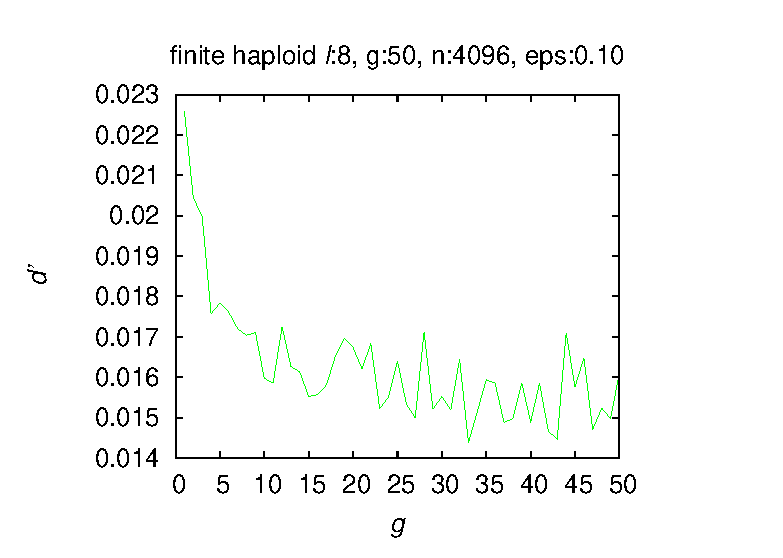
\includegraphics{figures/eps/vio/chi/b8/e0.1/n00004096_fin_hap.eps}}} \hspace{-3em}%
\subfloat{
\resizebox{8cm}{5cm}{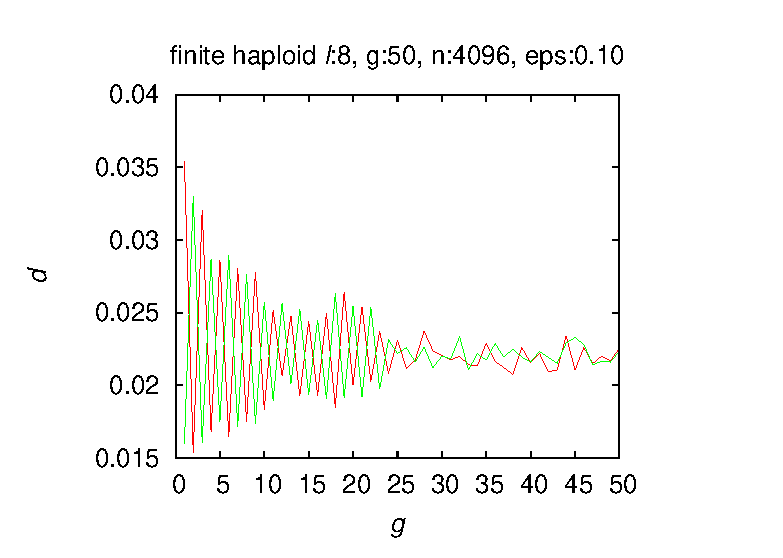
\includegraphics{figures/eps/vio/chi/b8/e0.1/n00004096_fin_hap_wovio.eps}}}\vspace{-1em} \hspace{-3em}%
\end{center}
\begin{center}
\subfloat{
\resizebox{8cm}{5cm}{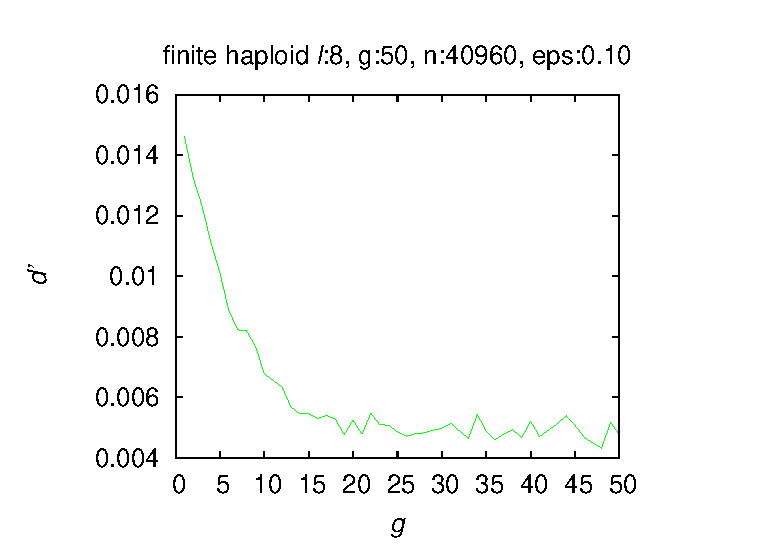
\includegraphics{figures/eps/vio/chi/b8/e0.1/n00040960_fin_hap.eps}}} \hspace{-3em}%
\subfloat{
\resizebox{8cm}{5cm}{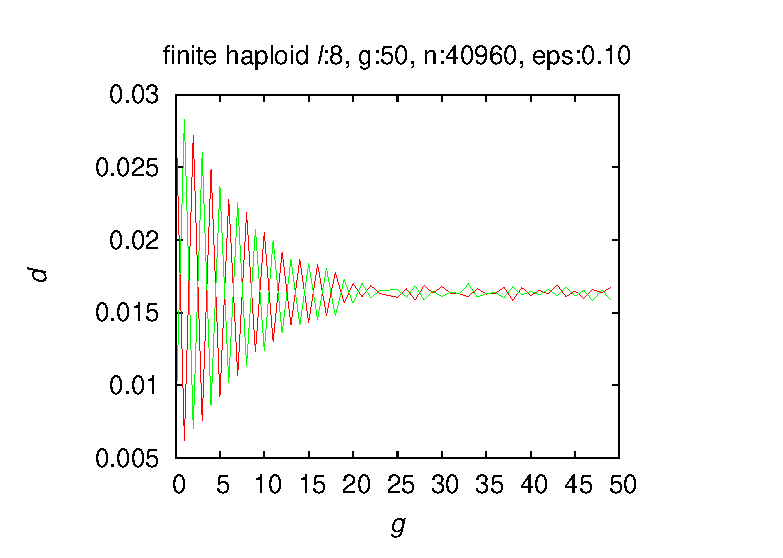
\includegraphics{figures/eps/vio/chi/b8/e0.1/n00040960_fin_hap_wovio.eps}}}\vspace{-1em} \hspace{-3em}%
\end{center}

\begin{center}
\subfloat{
\resizebox{8cm}{5cm}{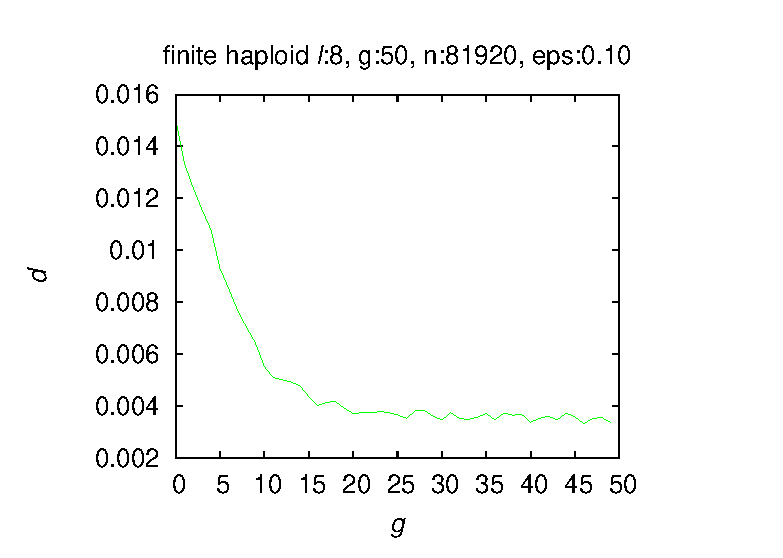
\includegraphics{figures/eps/vio/chi/b8/e0.1/n00081920_fin_hap.eps}}} \hspace{-3em}%
\subfloat{
\resizebox{8cm}{5cm}{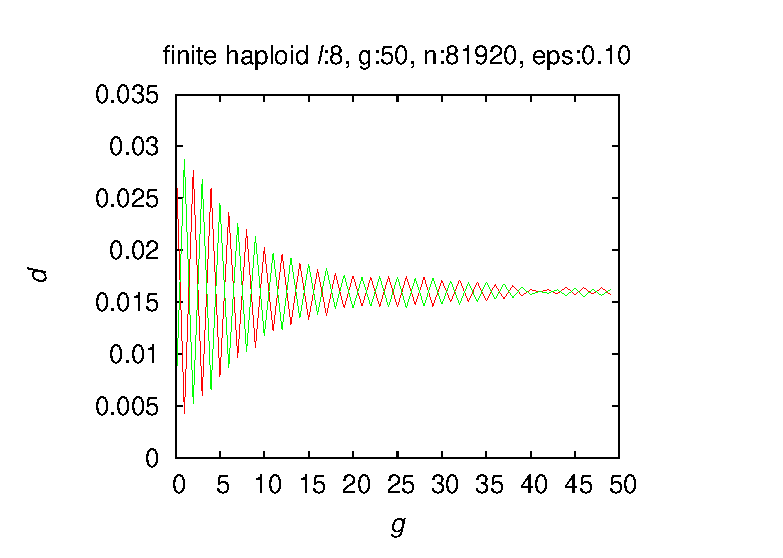
\includegraphics{figures/eps/vio/chi/b8/e0.1/n00081920_fin_hap_wovio.eps}}}\vspace{-1em} \hspace{-3em}%
\end{center}

\begin{center}
\subfloat{
\resizebox{8cm}{5cm}{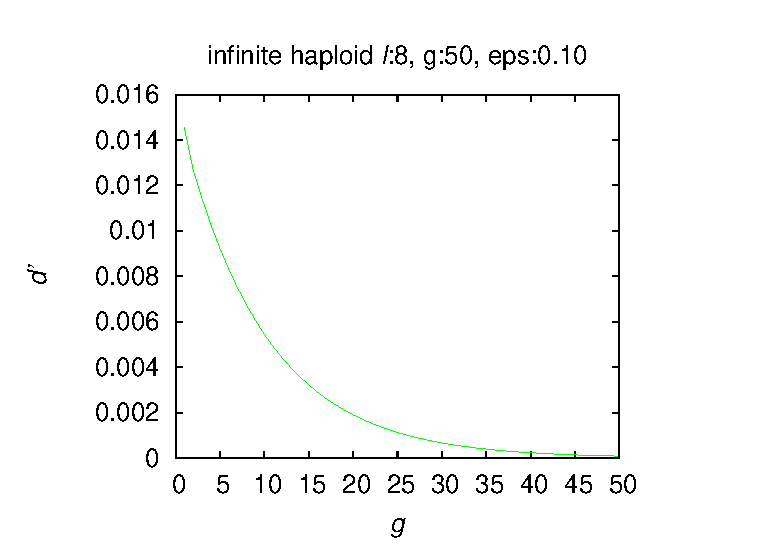
\includegraphics{figures/eps/vio/chi/b8/e0.1/inf_hap.eps}}}\hspace{-3em}%
\subfloat{
\resizebox{8cm}{5cm}{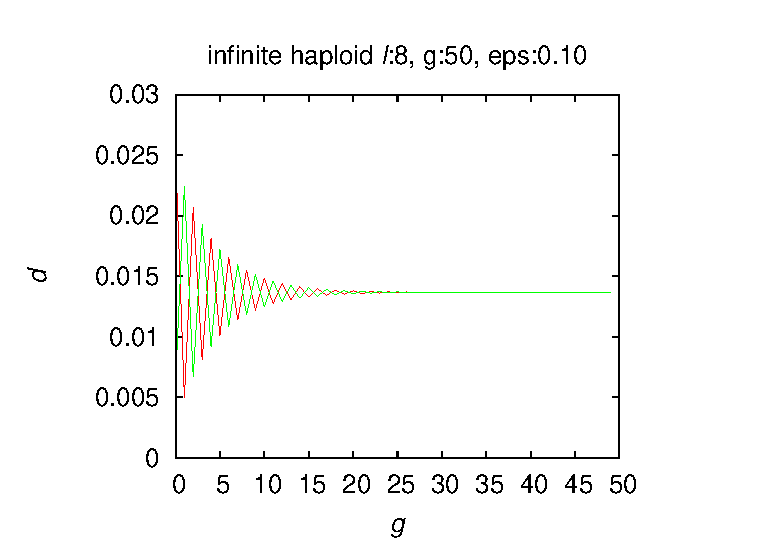
\includegraphics{figures/eps/vio/chi/b8/e0.1/inf_hap_wovio.eps}}}\vspace{-0.5em} \hspace{-3em}%


\caption{\textbf{Infinite and finite haploid population oscillation behavior in case of violation in $\bm{\chi}$ for genome length $\ell = 8$ and $\bm{\epsilon} = 0.1$:} 
  In left column, $d'$ is distance of finite population of size $n$ or infinite population to limit $\bm{z}^\ast$ for $g$ generations. In right column, $d$ is distance of finite population of size $N$ or infinite population to limits without violation.}
\label{oscillation_8h_vio_chi_0.1}
\end{center}
\end{figure}

% l = 10

\begin{figure}[h]
\begin{center}
\subfloat{
\resizebox{8cm}{5cm}{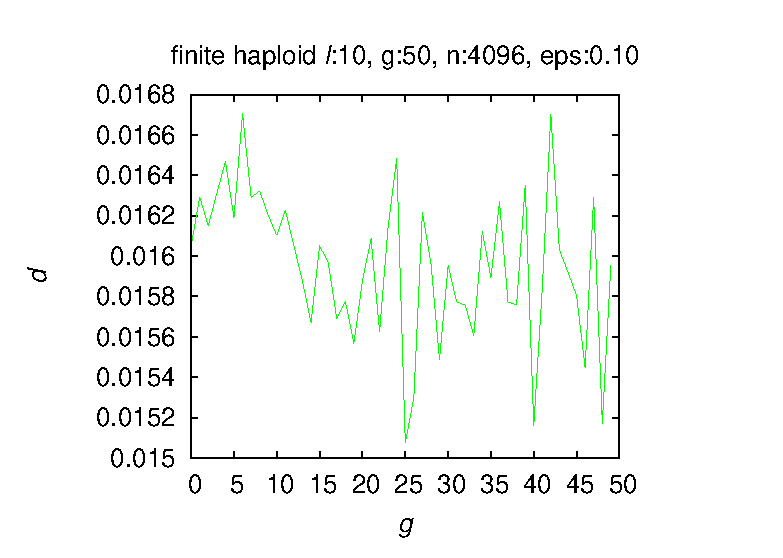
\includegraphics{figures/eps/vio/chi/b10/e0.1/n00004096_fin_hap.eps}}} \hspace{-3em}%
\subfloat{
\resizebox{8cm}{5cm}{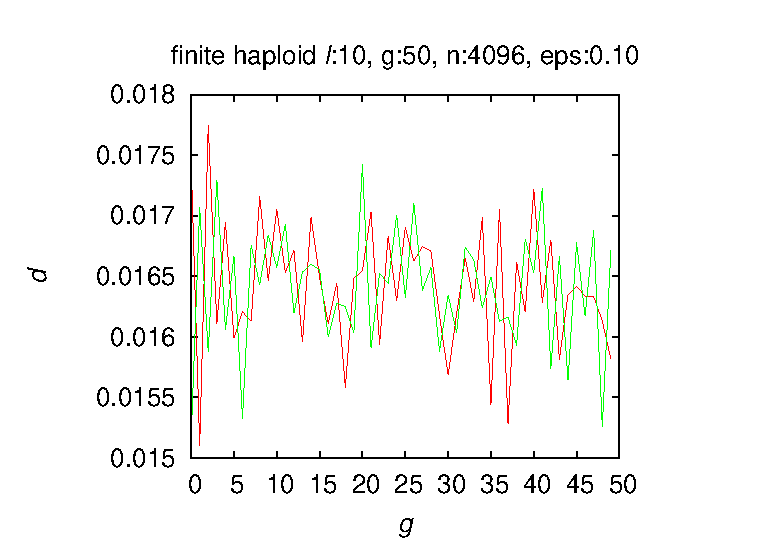
\includegraphics{figures/eps/vio/chi/b10/e0.1/n00004096_fin_hap_wovio.eps}}}\vspace{-1em} \hspace{-3em}%
\end{center}
\begin{center}
\subfloat{
\resizebox{8cm}{5cm}{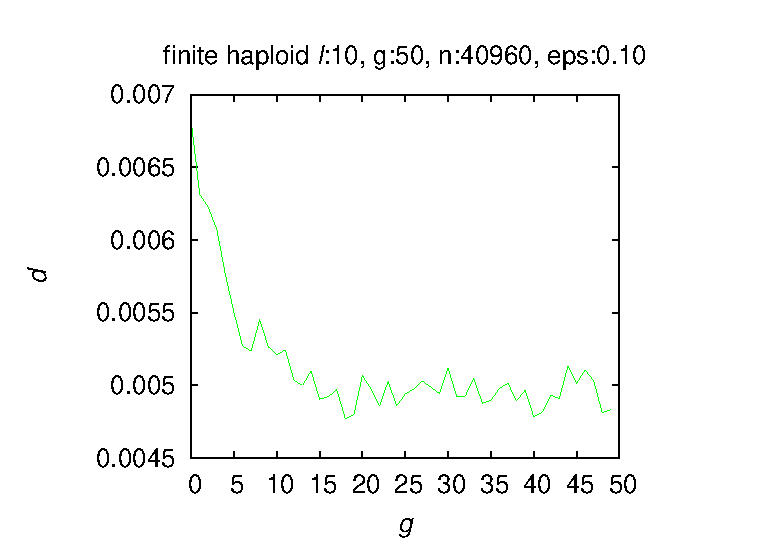
\includegraphics{figures/eps/vio/chi/b10/e0.1/n00040960_fin_hap.eps}}} \hspace{-3em}%
\subfloat{
\resizebox{8cm}{5cm}{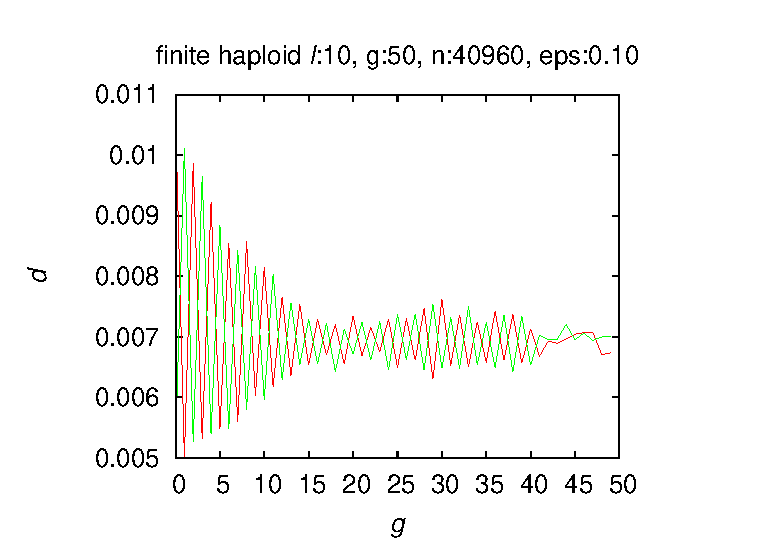
\includegraphics{figures/eps/vio/chi/b10/e0.1/n00040960_fin_hap_wovio.eps}}}\vspace{-1em} \hspace{-3em}%
\end{center}

\begin{center}
\subfloat{
\resizebox{8cm}{5cm}{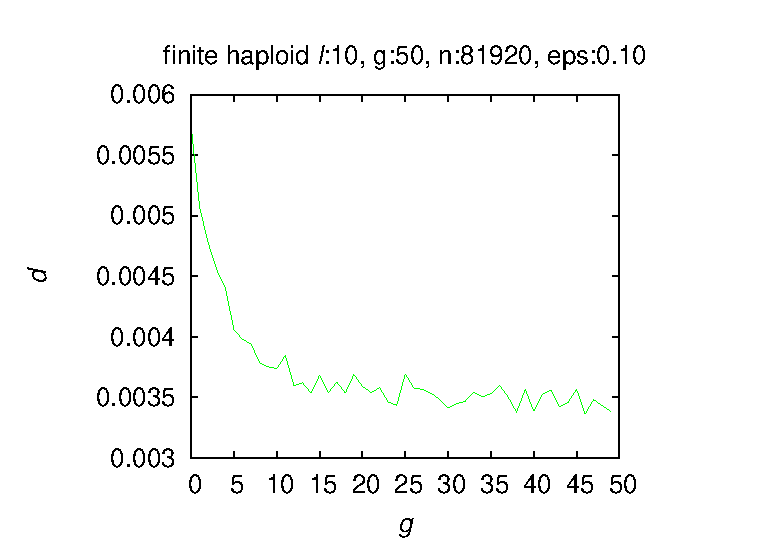
\includegraphics{figures/eps/vio/chi/b10/e0.1/n00081920_fin_hap.eps}}} \hspace{-3em}%
\subfloat{
\resizebox{8cm}{5cm}{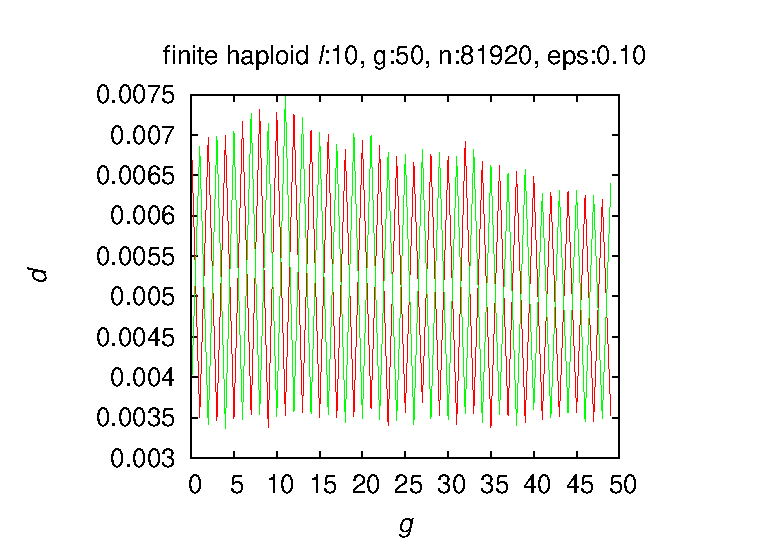
\includegraphics{figures/eps/vio/chi/b10/e0.1/n00081920_fin_hap_wovio.eps}}}\vspace{-1em} \hspace{-3em}%
\end{center}

\begin{center}
\subfloat{
\resizebox{8cm}{5cm}{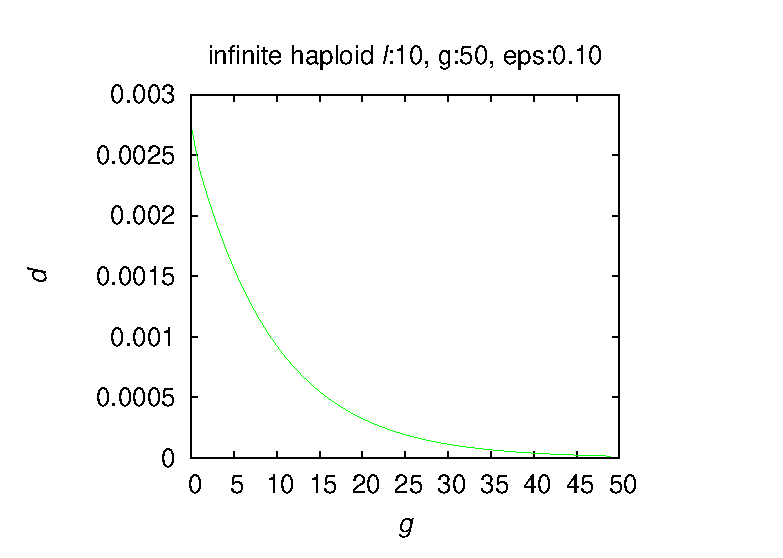
\includegraphics{figures/eps/vio/chi/b10/e0.1/inf_hap.eps}}}\hspace{-3em}%
\subfloat{
\resizebox{8cm}{5cm}{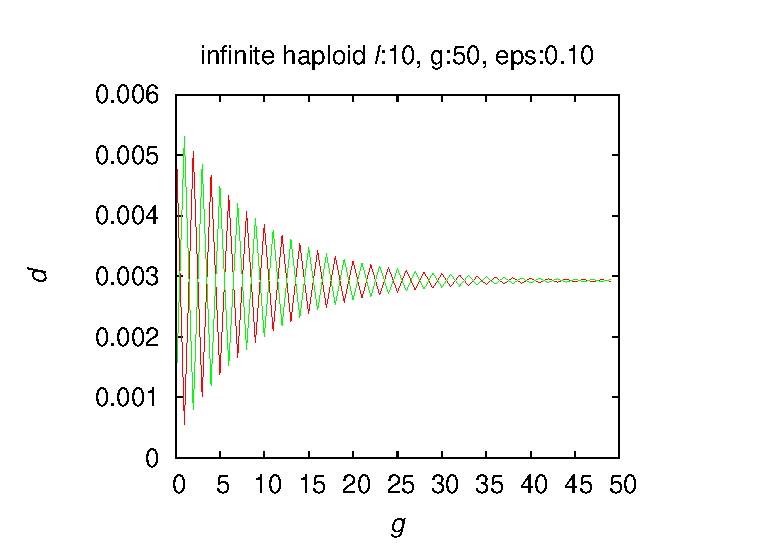
\includegraphics{figures/eps/vio/chi/b10/e0.1/inf_hap_wovio.eps}}}\vspace{-0.5em} \hspace{-3em}%

\caption{\textbf{Infinite and finite haploid population oscillation behavior in case of violation in $\bm{\chi}$ for genome length $\ell = 10$ and $\bm{\epsilon} = 0.1$:} 
  In left column, $d'$ is distance of finite population of size $n$ or infinite population to limit $\bm{z}^\ast$ for $g$ generations. In right column, $d$ is distance of finite population of size $N$ or infinite population to limits without violation.}
\label{oscillation_10h_vio_chi_0.1}
\end{center}
\end{figure}


% l = 12
\begin{figure}[h]
\begin{center}
\subfloat{
\resizebox{8cm}{5cm}{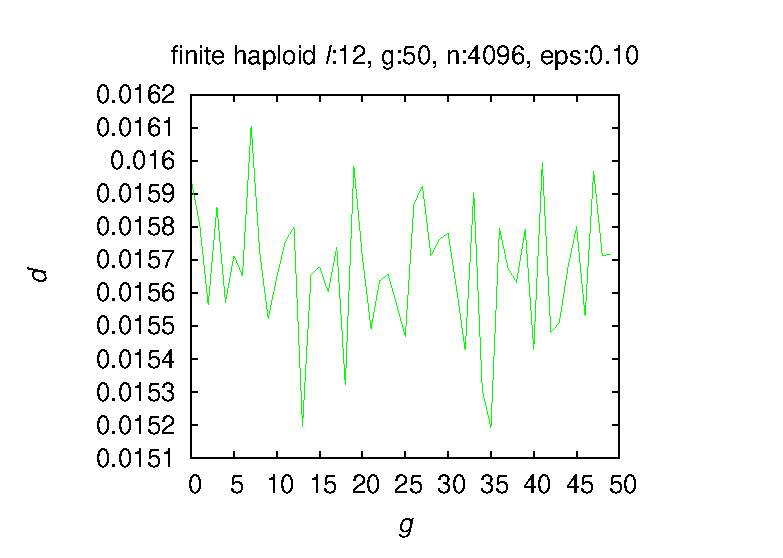
\includegraphics{figures/eps/vio/chi/b12/e0.1/n00004096_fin_hap.eps}}} \hspace{-3em}%
\subfloat{
\resizebox{8cm}{5cm}{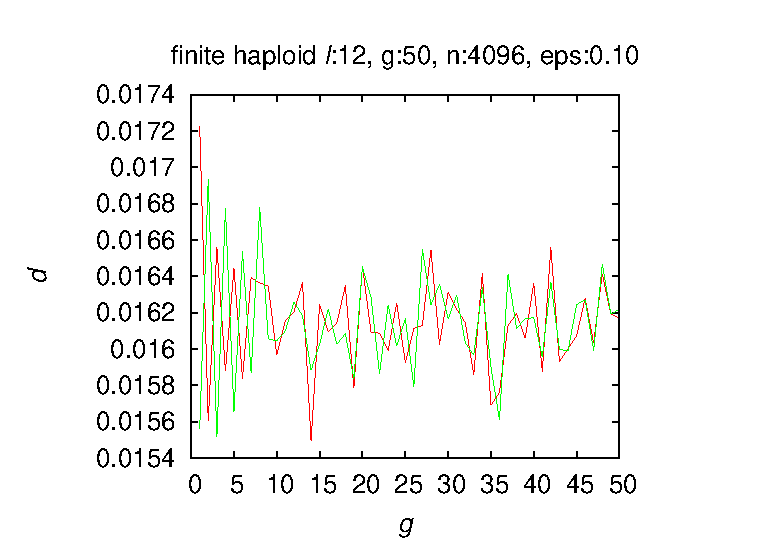
\includegraphics{figures/eps/vio/chi/b12/e0.1/n00004096_fin_hap_wovio.eps}}}\vspace{-1em} \hspace{-3em}%
\end{center}
\begin{center}
\subfloat{
\resizebox{8cm}{5cm}{\includegraphics{figures/eps/vio/chi/b12/e0.1/n00040960_fin_hap.eps}}} \hspace{-3em}%
\subfloat{
\resizebox{8cm}{5cm}{\includegraphics{figures/eps/vio/chi/b12/e0.1/n00040960_fin_hap_wovio.eps}}}\vspace{-1em} \hspace{-3em}%
\end{center}

\begin{center}
\subfloat{
\resizebox{8cm}{5cm}{\includegraphics{figures/eps/vio/chi/b12/e0.1/n00081920_fin_hap.eps}}} \hspace{-3em}%
\subfloat{
\resizebox{8cm}{5cm}{\includegraphics{figures/eps/vio/chi/b12/e0.1/n00081920_fin_hap_wovio.eps}}}\vspace{-1em} \hspace{-3em}%
\end{center}

\begin{center}
\subfloat{
\resizebox{8cm}{5cm}{\includegraphics{figures/eps/vio/chi/b12/e0.1/inf_hap.eps}}}\hspace{-3em}%
\subfloat{
\resizebox{8cm}{5cm}{\includegraphics{figures/eps/vio/chi/b12/e0.1/inf_hap_wovio.eps}}}\vspace{-0.5em} \hspace{-3em}%


\caption{\textbf{Infinite and finite haploid population oscillation behavior in case of violation in $\bm{\chi}$ for genome length $\ell = 12$ and $\bm{\epsilon} = 0.1$:} 
  In left column, $d'$ is distance of finite population of size $n$ or infinite population to limit $\bm{z}^\ast$ for $g$ generations. In right column, $d$ is distance of finite population of size $N$ or infinite population to limits without violation.}
\label{oscillation_12h_vio_chi_0.1}
\end{center}
\end{figure}

% l = 14

\begin{figure}[h]
\begin{center}
\subfloat{
\resizebox{8cm}{5cm}{\includegraphics{figures/eps/vio/chi/b14/e0.1/n00004096_fin_hap.eps}}} \hspace{-3em}%
\subfloat{
\resizebox{8cm}{5cm}{\includegraphics{figures/eps/vio/chi/b14/e0.1/n00004096_fin_hap_wovio.eps}}}\vspace{-1em} \hspace{-3em}%
\end{center}
\begin{center}
\subfloat{
\resizebox{8cm}{5cm}{\includegraphics{figures/eps/vio/chi/b14/e0.1/n00040960_fin_hap.eps}}} \hspace{-3em}%
\subfloat{
\resizebox{8cm}{5cm}{\includegraphics{figures/eps/vio/chi/b14/e0.1/n00040960_fin_hap_wovio.eps}}}\vspace{-1em} \hspace{-3em}%
\end{center}

\begin{center}
\subfloat{
\resizebox{8cm}{5cm}{\includegraphics{figures/eps/vio/chi/b14/e0.1/n00081920_fin_hap.eps}}} \hspace{-3em}%
\subfloat{
\resizebox{8cm}{5cm}{\includegraphics{figures/eps/vio/chi/b14/e0.1/n00081920_fin_hap_wovio.eps}}}\vspace{-1em} \hspace{-3em}%
\end{center}

\begin{center}
\subfloat{
\resizebox{8cm}{5cm}{\includegraphics{figures/eps/vio/chi/b14/e0.1/inf_hap.eps}}}\hspace{-3em}%
\subfloat{
\resizebox{8cm}{5cm}{\includegraphics{figures/eps/vio/chi/b14/e0.1/inf_hap_wovio.eps}}}\vspace{-0.5em} \hspace{-3em}%

\caption{\textbf{Infinite and finite haploid population oscillation behavior in case of violation in $\bm{\chi}$ for genome length $\ell = 14$ and $\bm{\epsilon} = 0.1$:} 
  In left column, $d'$ is distance of finite population of size $n$ or infinite population to limit $\bm{z}^\ast$ for $g$ generations. In right column, $d$ is distance of finite population of size $N$ or infinite population to limits without violation.}
\label{oscillation_14h_vio_chi_0.1}
\end{center}
\end{figure}

\clearpage

The right column in figures \ref{oscillation_8h_vio_chi_0.1} through \ref{oscillation_14h_vio_chi_0.1} 
shows distance of finite and infinite haploid populations to non-violation limits $\bm{p^\ast}$ and $\bm{q^\ast}$ with $\bm{\epsilon} \;=\; 0.1$. 
Graphs in the right column give picture of oscillating behavior of haploid population given violation. 
Both finite and infinite populations oscillate given violation, and oscillations amplitudes decreases with time. 
However, for $\bm{\epsilon} \;=\; 0.1$, oscillations in infinite populations die out quickly, 
but oscillations in finite populations did not die out completely. Rate of damping of ripples with $\bm{\epsilon} \;=\; 0.1$ is  
larger than with $\bm{\epsilon} \;=\; 0.01$. New masks created in crossover distribution with $\bm{\epsilon} \;=\; 0.1$ have still have small  
probability of being used during crossover for oscillation in finite populations to die out completely. 

The left column of figures \ref{oscillation_8h_vio_chi_0.1} through \ref{oscillation_14h_vio_chi_0.1} 
shows distance of finite and infinite haploid populations to limit $\bm{z^\ast}$ 
(limit with violation in crossover distribution $\bm{\chi}$) when $\bm{\epsilon} \;=\; 0.1$. 
The distance between finite population and limit $\bm{z}^\ast$ (limit with violation in $\bm{\chi}$ distribution) 
decreases as finite population size increases, 
and finite population shows behavior similar to infinite population behavior as finite population reach large number. 
The distance data for haploid population in case of violation in $\bm{\chi}$ distribution 
with $\bm{\epsilon} \;=\; 0.1$ for different finite population size $N$ are tabulated in table \ref{distanceChiHapEps0.1}.

\begin{table}[ht]
\caption{\textbf{Distance measured for violation in $\bm{\chi}$ with $\bm{\epsilon} \;=\; 0.1$  for haploids:} $\ell$ is genome length, 
average distance between finite and infinite population is tabulated in the last three columns, and last row is expected single step distance.}
\centering
\begin{tabularx}{0.75\textwidth}{ c *{3}{X}}
\toprule
$\ell$ & $N = 4096$ & $N = 40960$ & $N = 81920$  \\
\midrule
8 & 0.0163	& 0.0061 	& 0.0051 \\
10 & 0.0157	&  0.0051	& 0.0037 \\	
12 & 0.0157	&  0.0051	& 0.0037 \\	
14 & 0.0156	&  0.0049	& 0.0035 \\
\midrule
$1/\sqrt{N}$ & 0.0156 & 0.0049 & 0.0035 \\
\bottomrule
\end{tabularx}
\label{distanceChiHapEps0.1}
\end{table} 

From table \ref{distanceChiHapEps0.1}, average distance calculated for finite population size $4096$ is $0.0158$, 
for size $40960$ is $0.0053$ and for size $81920$ is $0.0038$. These results show average distance 
between finite population and limit $\bm{z^\ast}$ closely follows expected single step distance 
between finite and infinite population. The distance decreased as $1/\sqrt{N}$. 
Also, the distance decreased as genome length $\ell$ increased for all sizes of finite haploid populations 
with $\bm{\epsilon} \;=\; 0.1$.
 

\subsection{Haploid Population $\mathtt{\sim}$ $\epsilon: 0.5$}

% l = 8

\begin{figure}[h]
\begin{center}
\subfloat{
\resizebox{8cm}{5cm}{\includegraphics{figures/eps/vio/chi/b8/e0.5/n00004096_fin_hap.eps}}} \hspace{-3em}%
\subfloat{
\resizebox{8cm}{5cm}{\includegraphics{figures/eps/vio/chi/b8/e0.5/n00004096_fin_hap_wovio.eps}}}\vspace{-1em} \hspace{-3em}%
\end{center}
\begin{center}
\subfloat{
\resizebox{8cm}{5cm}{\includegraphics{figures/eps/vio/chi/b8/e0.5/n00040960_fin_hap.eps}}} \hspace{-3em}%
\subfloat{
\resizebox{8cm}{5cm}{\includegraphics{figures/eps/vio/chi/b8/e0.5/n00040960_fin_hap_wovio.eps}}}\vspace{-1em} \hspace{-3em}%
\end{center}

\begin{center}
\subfloat{
\resizebox{8cm}{5cm}{\includegraphics{figures/eps/vio/chi/b8/e0.5/n00081920_fin_hap.eps}}} \hspace{-3em}%
\subfloat{
\resizebox{8cm}{5cm}{\includegraphics{figures/eps/vio/chi/b8/e0.5/n00081920_fin_hap_wovio.eps}}}\vspace{-1em} \hspace{-3em}%
\end{center}

\begin{center}
\subfloat{
\resizebox{8cm}{5cm}{\includegraphics{figures/eps/vio/chi/b8/e0.5/inf_hap.eps}}}\hspace{-3em}%
\subfloat{
\resizebox{8cm}{5cm}{\includegraphics{figures/eps/vio/chi/b8/e0.5/inf_hap_wovio.eps}}}\vspace{-0.5em} \hspace{-3em}%


\caption{\textbf{Infinite and finite haploid population oscillation behavior in case of violation in $\bm{\chi}$ for genome length $\ell = 8$ and $\bm{\epsilon} = 0.5$:} 
  In left column, $d'$ is distance of finite population of size $n$ or infinite population to limit $\bm{z}^\ast$ for $g$ generations. In right column, $d$ is distance of finite population or infinite population to limits $\bm{p}^\ast$ and $\bm{q}^\ast$ without violation.}
\label{oscillation_8h_vio_chi_0.5}
\end{center}
\end{figure}


% l = 10

\begin{figure}[h]
\begin{center}
\subfloat{
\resizebox{8cm}{5cm}{\includegraphics{figures/eps/vio/chi/b10/e0.5/n00004096_fin_hap.eps}}} \hspace{-3em}%
\subfloat{
\resizebox{8cm}{5cm}{\includegraphics{figures/eps/vio/chi/b10/e0.5/n00004096_fin_hap_wovio.eps}}}\vspace{-1em} \hspace{-3em}%
\end{center}
\begin{center}
\subfloat{
\resizebox{8cm}{5cm}{\includegraphics{figures/eps/vio/chi/b10/e0.5/n00040960_fin_hap.eps}}} \hspace{-3em}%
\subfloat{
\resizebox{8cm}{5cm}{\includegraphics{figures/eps/vio/chi/b10/e0.5/n00040960_fin_hap_wovio.eps}}}\vspace{-1em} \hspace{-3em}%
\end{center}

\begin{center}
\subfloat{
\resizebox{8cm}{5cm}{\includegraphics{figures/eps/vio/chi/b10/e0.5/n00081920_fin_hap.eps}}} \hspace{-3em}%
\subfloat{
\resizebox{8cm}{5cm}{\includegraphics{figures/eps/vio/chi/b10/e0.5/n00081920_fin_hap_wovio.eps}}}\vspace{-1em} \hspace{-3em}%
\end{center}

\begin{center}
\subfloat{
\resizebox{8cm}{5cm}{\includegraphics{figures/eps/vio/chi/b10/e0.5/inf_hap.eps}}}\hspace{-3em}%
\subfloat{
\resizebox{8cm}{5cm}{\includegraphics{figures/eps/vio/chi/b10/e0.5/inf_hap_wovio.eps}}}\vspace{-0.5em} \hspace{-3em}%

\caption{\textbf{Infinite and finite haploid population oscillation behavior in case of violation in $\bm{\chi}$ for genome length $\ell = 10$ and $\bm{\epsilon} = 0.5$:} 
  In left column, $d'$ is distance of finite population of size $n$ or infinite population to limit $\bm{z}^\ast$ for $g$ generations. In right column, $d$ is distance of finite population or infinite population to limits $\bm{p}^\ast$ and $\bm{q}^\ast$ without violation.}
\label{oscillation_10h_vio_chi_0.5}
\end{center}
\end{figure}

% l = 12
\begin{figure}[h]
\begin{center}
\subfloat{
\resizebox{8cm}{5cm}{\includegraphics{figures/eps/vio/chi/b12/e0.5/n00004096_fin_hap.eps}}} \hspace{-3em}%
\subfloat{
\resizebox{8cm}{5cm}{\includegraphics{figures/eps/vio/chi/b12/e0.5/n00004096_fin_hap_wovio.eps}}}\vspace{-1em} \hspace{-3em}%
\end{center}
\begin{center}
\subfloat{
\resizebox{8cm}{5cm}{\includegraphics{figures/eps/vio/chi/b12/e0.5/n00040960_fin_hap.eps}}} \hspace{-3em}%
\subfloat{
\resizebox{8cm}{5cm}{\includegraphics{figures/eps/vio/chi/b12/e0.5/n00040960_fin_hap_wovio.eps}}}\vspace{-1em} \hspace{-3em}%
\end{center}

\begin{center}
\subfloat{
\resizebox{8cm}{5cm}{\includegraphics{figures/eps/vio/chi/b12/e0.5/n00081920_fin_hap.eps}}} \hspace{-3em}%
\subfloat{
\resizebox{8cm}{5cm}{\includegraphics{figures/eps/vio/chi/b12/e0.5/n00081920_fin_hap_wovio.eps}}}\vspace{-1em} \hspace{-3em}%
\end{center}

\begin{center}
\subfloat{
\resizebox{8cm}{5cm}{\includegraphics{figures/eps/vio/chi/b12/e0.5/inf_hap.eps}}}\hspace{-3em}%
\subfloat{
\resizebox{8cm}{5cm}{\includegraphics{figures/eps/vio/chi/b12/e0.5/inf_hap_wovio.eps}}}\vspace{-0.5em} \hspace{-3em}%


\caption{\textbf{Infinite and finite haploid population oscillation behavior in case of violation in $\bm{\chi}$ for genome length $\ell = 12$ and $\bm{\epsilon} = 0.5$:} 
  In left column, $d'$ is distance of finite population of size $n$ or infinite population to limit $\bm{z}^\ast$ for $g$ generations. In right column, $d$ is distance of finite population or infinite population to limits $\bm{p}^\ast$ and $\bm{q}^\ast$ without violation.}
\label{oscillation_12h_vio_chi_0.5}
\end{center}
\end{figure}

% l = 14

\begin{figure}[h]
\begin{center}
\subfloat{
\resizebox{8cm}{5cm}{\includegraphics{figures/eps/vio/chi/b14/e0.5/n00004096_fin_hap.eps}}} \hspace{-3em}%
\subfloat{
\resizebox{8cm}{5cm}{\includegraphics{figures/eps/vio/chi/b14/e0.5/n00004096_fin_hap_wovio.eps}}}\vspace{-1em} \hspace{-3em}%
\end{center}
\begin{center}
\subfloat{
\resizebox{8cm}{5cm}{\includegraphics{figures/eps/vio/chi/b14/e0.5/n00040960_fin_hap.eps}}} \hspace{-3em}%
\subfloat{
\resizebox{8cm}{5cm}{\includegraphics{figures/eps/vio/chi/b14/e0.5/n00040960_fin_hap_wovio.eps}}}\vspace{-1em} \hspace{-3em}%
\end{center}

\begin{center}
\subfloat{
\resizebox{8cm}{5cm}{\includegraphics{figures/eps/vio/chi/b14/e0.5/n00081920_fin_hap.eps}}} \hspace{-3em}%
\subfloat{
\resizebox{8cm}{5cm}{\includegraphics{figures/eps/vio/chi/b14/e0.5/n00081920_fin_hap_wovio.eps}}}\vspace{-1em} \hspace{-3em}%
\end{center}

\begin{center}
\subfloat{
\resizebox{8cm}{5cm}{\includegraphics{figures/eps/vio/chi/b14/e0.5/inf_hap.eps}}}\hspace{-3em}%
\subfloat{
\resizebox{8cm}{5cm}{\includegraphics{figures/eps/vio/chi/b14/e0.5/inf_hap_wovio.eps}}}\vspace{-0.5em} \hspace{-3em}%

\caption{\textbf{Infinite and finite haploid population oscillation behavior in case of violation in $\bm{\chi}$ for genome length $\ell = 14$ and $\bm{\epsilon} = 0.5$:} 
  In left column, $d'$ is distance of finite population of size $n$ or infinite population to limit $\bm{z}^\ast$ for $g$ generations. In right column, $d$ is distance of finite population or infinite population to limits $\bm{p}^\ast$ and $\bm{q}^\ast$ without violation.}
\label{oscillation_14h_vio_chi_0.5}
\end{center}
\end{figure}

\clearpage

The right column in figures \ref{oscillation_8h_vio_chi_0.5} through \ref{oscillation_14h_vio_chi_0.5} 
shows distance of finite and infinite haploid populations to non-violation limits $\bm{p^\ast}$ and $\bm{q^\ast}$ with $\bm{\epsilon} \;=\; 0.5$. 
The graphs indicate oscillating behavior of haploid population given violation. 
Unlike mutation with violation $\bm{\epsilon} \;=\; 0.5$, absence of oscillation is not observed. 
Finite populations still show some though not very clear oscillations, and infinite populations also oscillate but the oscillation dies out quickly. 

The left column of figures \ref{oscillation_8h_vio_chi_0.5} through \ref{oscillation_14h_vio_chi_0.5} 
shows distance of finite and infinite haploid populations to limit $\bm{z^\ast}$ 
(limit with violation in crossover distribution $\bm{\chi}$) when $\bm{\epsilon} \;=\; 0.5$. 
The distance between finite population and limit $\bm{z}^\ast$ (limit with violation in $\bm{\chi}$ distribution) 
decreases as finite population size increases, 
and finite population shows behavior similar to infinite population behavior as finite population size grows. 
Average distance data for haploid population in case of violation in $\bm{\chi}$ distribution 
with $\bm{\epsilon} \;=\; 0.5$ for different finite population size $N$ are tabulated in table \ref{distanceChiHapEps0.5}. 

\begin{table}[ht]
\caption{\textbf{Distance measured for violation in $\bm{\chi}$ with $\bm{\epsilon} \;=\; 0.5$  for haploids:} $\ell$ is genome length, 
average distance between finite and infinite population is tabulated in the last three columns, and last row is expected single step distance.}
\centering
\begin{tabularx}{0.75\textwidth}{ c *{3}{X}}
\toprule
$\ell$ & $N = 4096$ & $N = 40960$ & $N = 81920$  \\
\midrule
8 & 0.0156	&  0.0051	& 0.0036 \\
10 & 0.0155	&  0.0049	& 0.0035 \\
12 & 0.0157	&  0.0050	& 0.0035 \\
14 & 0.0156	&  0.0049	& 0.0035 \\      
\midrule
$1/\sqrt{N}$ & 0.0156 & 0.0049 & 0.0035 \\
\bottomrule
\end{tabularx}
\label{distanceChiHapEps0.5}
\end{table} 

The results from Table \ref{distanceChiHapEps0.5} show average distance 
between finite population and limit $\bm{z^\ast}$ approaches expected single step distance 
between finite and infinite population. The distance decreased as $1/\sqrt{N}$. 









\clearpage
\subsection{Diploid Population $\mathtt{\sim}$ $\epsilon: 0.01$}
% l = 8
% \mbox{}\\[-0.75in]
\begin{figure}[!b]
\begin{center}
\subfloat{
\resizebox{8cm}{4.5cm}{\includegraphics{figures/eps/vio/chi/b8/e0.01/n00004096_fin_dip.eps}}}\hspace{-3em}%
\subfloat{
\resizebox{8cm}{4.5cm}{\includegraphics{figures/eps/vio/chi/b8/e0.01/n00004096_fin_dip_wovio.eps}}}\vspace{-1em}  \hspace{-3em}%
\end{center}
\begin{center}
\subfloat{
\resizebox{8cm}{4.5cm}{\includegraphics{figures/eps/vio/chi/b8/e0.01/n00040960_fin_dip.eps}}}\hspace{-3em}%
\subfloat{
\resizebox{8cm}{4.5cm}{\includegraphics{figures/eps/vio/chi/b8/e0.01/n00040960_fin_dip_wovio.eps}}}\vspace{-1em}  \hspace{-3em}%
\end{center}


\begin{center}
\subfloat{
\resizebox{8cm}{4.5cm}{\includegraphics{figures/eps/vio/chi/b8/e0.01/n00081920_fin_dip.eps}}}\hspace{-3em}%
\subfloat{
\resizebox{8cm}{4.5cm}{\includegraphics{figures/eps/vio/chi/b8/e0.01/n00081920_fin_dip_wovio.eps}}}\vspace{-1em}  \hspace{-3em}%
\end{center}

\begin{center}
\subfloat{
\resizebox{8cm}{4.5cm}{\includegraphics{figures/eps/vio/chi/b8/e0.01/inf_dip.eps}}}\hspace{-3em}%
\subfloat{
\resizebox{8cm}{4.5cm}{\includegraphics{figures/eps/vio/chi/b8/e0.01/inf_dip_wovio.eps}}}\vspace{-0.5em}  \hspace{-3em}%


\caption[\textbf{Infinite and finite diploid population behavior for $\bm{\chi}$ violation, $\ell = 8$ and $\bm{\epsilon} = 0.01$}]
{\textbf{Infinite and finite diploid population behavior for $\bm{\chi}$ violation, $\ell = 8$ and $\bm{\epsilon} = 0.01$:} 
  In left column, $d'$ is distance of finite or infinite population to limit $\bm{z}^\ast$ for $g$ generations. 
  In right column, $d$ is distance of finite or infinite population to limits $\bm{p}^\ast$ and $\bm{q}^\ast$. Green line is distance to $\bm{p}^\ast$ and red line is distance to $\bm{q}^\ast$.}
\label{oscillation_8d_vio_chi_0.01}
\end{center}
\end{figure}

% l = 10

\begin{figure}[h]
\begin{center}
\subfloat{
\resizebox{8cm}{4.5cm}{\includegraphics{figures/eps/vio/chi/b10/e0.01/n00004096_fin_dip.eps}}}\hspace{-3em}%
\subfloat{
\resizebox{8cm}{4.5cm}{\includegraphics{figures/eps/vio/chi/b10/e0.01/n00004096_fin_dip_wovio.eps}}}\vspace{-1em}  \hspace{-3em}%
\end{center}
\begin{center}
\subfloat{
\resizebox{8cm}{4.5cm}{\includegraphics{figures/eps/vio/chi/b10/e0.01/n00040960_fin_dip.eps}}}\hspace{-3em}%
\subfloat{
\resizebox{8cm}{4.5cm}{\includegraphics{figures/eps/vio/chi/b10/e0.01/n00040960_fin_dip_wovio.eps}}}\vspace{-1em}  \hspace{-3em}%
\end{center}


\begin{center}
\subfloat{
\resizebox{8cm}{4.5cm}{\includegraphics{figures/eps/vio/chi/b10/e0.01/n00081920_fin_dip.eps}}}\hspace{-3em}%
\subfloat{
\resizebox{8cm}{4.5cm}{\includegraphics{figures/eps/vio/chi/b10/e0.01/n00081920_fin_dip_wovio.eps}}}\vspace{-1em}  \hspace{-3em}%
\end{center}

\begin{center}
\subfloat{
\resizebox{8cm}{4.5cm}{\includegraphics{figures/eps/vio/chi/b10/e0.01/inf_dip.eps}}}\hspace{-3em}%
\subfloat{
\resizebox{8cm}{4.5cm}{\includegraphics{figures/eps/vio/chi/b10/e0.01/inf_dip_wovio.eps}}}\vspace{-0.5em}  \hspace{-3em}%


\caption[\textbf{Infinite and finite diploid population behavior for $\bm{\chi}$ violation $\bm{\chi}$, genome length $\ell = 10$ and $\bm{\epsilon} = 0.01$}]{\textbf{Infinite and finite diploid population behavior for $\bm{\chi}$ violation, genome length $\ell = 10$ and $\bm{\epsilon} = 0.01$:} 
  In left column, $d'$ is distance of finite or infinite population to limit $\bm{z}^\ast$ for $g$ generations. In right column, $d$ is distance of finite or infinite population to limits $\bm{p}^\ast$ and $\bm{q}^\ast$. Green line is distance to $\bm{p}^\ast$ and red line is distance to $\bm{q}^\ast$.}
\label{oscillation_10d_vio_chi_0.01}
\end{center}
\end{figure}

% l = 12

\begin{figure}[h]
\begin{center}
\subfloat{
\resizebox{8cm}{4.5cm}{\includegraphics{figures/eps/vio/chi/b12/e0.01/n00004096_fin_dip.eps}}}\hspace{-3em}%
\subfloat{
\resizebox{8cm}{4.5cm}{\includegraphics{figures/eps/vio/chi/b12/e0.01/n00004096_fin_dip_wovio.eps}}}\vspace{-1em}  \hspace{-3em}%
\end{center}
\begin{center}
\subfloat{
\resizebox{8cm}{4.5cm}{\includegraphics{figures/eps/vio/chi/b12/e0.01/n00040960_fin_dip.eps}}}\hspace{-3em}%
\subfloat{
\resizebox{8cm}{4.5cm}{\includegraphics{figures/eps/vio/chi/b12/e0.01/n00040960_fin_dip_wovio.eps}}}\vspace{-1em}  \hspace{-3em}%
\end{center}


\begin{center}
\subfloat{
\resizebox{8cm}{4.5cm}{\includegraphics{figures/eps/vio/chi/b12/e0.01/n00081920_fin_dip.eps}}}\hspace{-3em}%
\subfloat{
\resizebox{8cm}{4.5cm}{\includegraphics{figures/eps/vio/chi/b12/e0.01/n00081920_fin_dip_wovio.eps}}}\vspace{-1em}  \hspace{-3em}%
\end{center}

\begin{center}
\subfloat{
\resizebox{8cm}{4.5cm}{\includegraphics{figures/eps/vio/chi/b12/e0.01/inf_dip.eps}}}\hspace{-3em}%
\subfloat{
\resizebox{8cm}{4.5cm}{\includegraphics{figures/eps/vio/chi/b12/e0.01/inf_dip_wovio.eps}}}\vspace{-0.5em}  \hspace{-3em}%


\caption[\textbf{Infinite and finite diploid population behavior for $\bm{\chi}$ violation, genome length $\ell = 12$ and $\bm{\epsilon} = 0.01$}]{\textbf{Infinite and finite diploid population behavior for  $\bm{\chi}$ violation, genome length $\ell = 12$ and $\bm{\epsilon} = 0.01$:} 
  In left column, $d'$ is distance of finite or infinite population to limit $\bm{z}^\ast$ for $g$ generations. In right column, $d$ is distance of finite or infinite population to limits $\bm{p}^\ast$ and $\bm{q}^\ast$. Green line is distance to $\bm{p}^\ast$ and red line is distance to $\bm{q}^\ast$.}
\label{oscillation_12d_vio_chi_0.01}
\end{center}
\end{figure}

% l = 14

\begin{figure}[h]
\begin{center}
\subfloat{
\resizebox{8cm}{4.5cm}{\includegraphics{figures/eps/vio/chi/b14/e0.01/n00004096_fin_dip.eps}}}\hspace{-3em}%
\subfloat{
\resizebox{8cm}{4.5cm}{\includegraphics{figures/eps/vio/chi/b14/e0.01/n00004096_fin_dip_wovio.eps}}}\vspace{-1em}  \hspace{-3em}%
\end{center}
\begin{center}
\subfloat{
\resizebox{8cm}{4.5cm}{\includegraphics{figures/eps/vio/chi/b14/e0.01/n00040960_fin_dip.eps}}}\hspace{-3em}%
\subfloat{
\resizebox{8cm}{4.5cm}{\includegraphics{figures/eps/vio/chi/b14/e0.01/n00040960_fin_dip_wovio.eps}}}\vspace{-1em}  \hspace{-3em}%
\end{center}


\begin{center}
\subfloat{
\resizebox{8cm}{4.5cm}{\includegraphics{figures/eps/vio/chi/b14/e0.01/n00081920_fin_dip.eps}}}\hspace{-3em}%
\subfloat{
\resizebox{8cm}{4.5cm}{\includegraphics{figures/eps/vio/chi/b14/e0.01/n00081920_fin_dip_wovio.eps}}}\vspace{-1em}  \hspace{-3em}%
\end{center}

\begin{center}
\subfloat{
\resizebox{8cm}{4.5cm}{\includegraphics{figures/eps/vio/chi/b14/e0.01/inf_dip.eps}}}\hspace{-3em}%
\subfloat{
\resizebox{8cm}{4.5cm}{\includegraphics{figures/eps/vio/chi/b14/e0.01/inf_dip_wovio.eps}}}\vspace{-0.5em}  \hspace{-3em}%


\caption[\textbf{Infinite and finite diploid population behavior for  $\bm{\chi}$ violation, genome length $\ell = 14$ and $\bm{\epsilon} = 0.01$}]{\textbf{Infinite and finite diploid population behavior for  $\bm{\chi}$ violation, genome length $\ell = 14$ and $\bm{\epsilon} = 0.01$:} 
  In left column, $d'$ is distance of finite or infinite population to limit $\bm{z}^\ast$ for $g$ generations. In right column, $d$ is distance of finite or infinite population to limits $\bm{p}^\ast$ and $\bm{q}^\ast$. Green line is distance to $\bm{p}^\ast$ and red line is distance to $\bm{q}^\ast$.}
\label{oscillation_14d_vio_chi_0.01}
\end{center}
\end{figure}

% \clearpage
The right column in figures \ref{oscillation_8d_vio_chi_0.01} through \ref{oscillation_14d_vio_chi_0.01} 
shows distance of finite and infinite diploid populations to non-violation limits $\bm{p^\ast}$ and $\bm{q^\ast}$ with $\bm{\epsilon} \;=\; 0.01$. 
Those graphs indicate oscillating behavior. 
Since $\bm{\epsilon}$ 
is small, damping of ripples is slow. 
Infinite population oscillation does not die out in 50 generations 
even though it dies out eventually. 
Finite population graphs show randomness, and oscillation improves with increased population size.
That can be noticed more clearly in figures \ref{oscillation_12d_vio_chi_0.01} and \ref{oscillation_14d_vio_chi_0.01}.

The left column of figures \ref{oscillation_8d_vio_chi_0.01} through \ref{oscillation_14d_vio_chi_0.01} 
shows distance of finite and infinite diploid populations to limit $\bm{z^\ast}$ 
(limit with violation in crossover distribution $\bm{\chi}$) when $\bm{\epsilon} \;=\; 0.01$. 
The distance decreases as population size increases. 
Average distance data for diploid population in case of violation in $\bm{\chi}$ distribution 
with $\bm{\epsilon} \;=\; 0.01$ for different finite population size $N$ are tabulated in table \ref{distanceChiDipEps0.01}.

Table \ref{distanceChiDipEps0.01} shows that the average distance 
between finite and infinite population approaches the expected single step distance $1/\sqrt{N}$. 

\clearpage
\begin{table}[h]
\caption[\textbf{Distance measured for violation in $\bm{\chi}$ with $\bm{\epsilon} \;=\; 0.01$ diploids}]{\textbf{Distance measured for violation in $\bm{\chi}$ with $\bm{\epsilon} \;=\; 0.01$ diploids:} $\ell$ is genome length, 
average distance between finite and infinite population is tabulated in the last three columns, and last row is expected single step distance.}
\centering
\begin{tabularx}{0.75\textwidth}{ c *{3}{X}}
\toprule
$\ell$ & $N = 4096$ & $N = 40960$ & $N = 81920$  \\
\midrule
8 & 0.0156	&  0.0051	& 0.0036 \\
10 & 0.0156	&  0.0049	& 0.0035 \\
12 & 0.0156	&  0.0049	& 0.0035 \\
14 & 0.0156	&  0.0049	& 0.0035 \\
\midrule
$1/\sqrt{N}$ & 0.0156 & 0.0049 & 0.0035 \\
\bottomrule
\end{tabularx}
\label{distanceChiDipEps0.01}
\end{table} 


\clearpage
\subsection{Diploid Population $\mathtt{\sim}$ $\epsilon: 0.1$}
% l = 8
\begin{figure}[h]
\begin{center}
\subfloat{
\resizebox{8cm}{5cm}{\includegraphics{figures/eps/vio/chi/b8/e0.1/n00004096_fin_dip.eps}}}\hspace{-3em}%
\subfloat{
\resizebox{8cm}{5cm}{\includegraphics{figures/eps/vio/chi/b8/e0.1/n00004096_fin_dip_wovio.eps}}}\vspace{-1em}  \hspace{-3em}%
\end{center}
\begin{center}
\subfloat{
\resizebox{8cm}{5cm}{\includegraphics{figures/eps/vio/chi/b8/e0.1/n00040960_fin_dip.eps}}}\hspace{-3em}%
\subfloat{
\resizebox{8cm}{5cm}{\includegraphics{figures/eps/vio/chi/b8/e0.1/n00040960_fin_dip_wovio.eps}}}\vspace{-1em}  \hspace{-3em}%
\end{center}


\begin{center}
\subfloat{
\resizebox{8cm}{5cm}{\includegraphics{figures/eps/vio/chi/b8/e0.1/n00081920_fin_dip.eps}}}\hspace{-3em}%
\subfloat{
\resizebox{8cm}{5cm}{\includegraphics{figures/eps/vio/chi/b8/e0.1/n00081920_fin_dip_wovio.eps}}}\vspace{-1em}  \hspace{-3em}%
\end{center}

\begin{center}
\subfloat{
\resizebox{8cm}{5cm}{\includegraphics{figures/eps/vio/chi/b8/e0.1/inf_dip.eps}}}\hspace{-3em}%
\subfloat{
\resizebox{8cm}{5cm}{\includegraphics{figures/eps/vio/chi/b8/e0.1/inf_dip_wovio.eps}}}\vspace{-0.5em}  \hspace{-3em}%


\caption{\textbf{Infinite and finite diploid population oscillation behavior in case of violation in $\bm{\chi}$ for genome length $\ell = 8$ and $\bm{\epsilon} = 0.1$:} 
  In left column, $d'$ is distance of finite population of size $n$ or infinite population to limit $\bm{z}^\ast$ for $g$ generations. In right column, $d$ is distance of finite population or infinite population to limits $\bm{p}^\ast$ and $\bm{q}^\ast$ without violation.}
\label{oscillation_8d_vio_chi_0.1}
\end{center}
\end{figure}

% l = 10

\begin{figure}[h]
\begin{center}
\subfloat{
\resizebox{8cm}{5cm}{\includegraphics{figures/eps/vio/chi/b10/e0.1/n00004096_fin_dip.eps}}}\hspace{-3em}%
\subfloat{
\resizebox{8cm}{5cm}{\includegraphics{figures/eps/vio/chi/b10/e0.1/n00004096_fin_dip_wovio.eps}}}\vspace{-1em}  \hspace{-3em}%
\end{center}
\begin{center}
\subfloat{
\resizebox{8cm}{5cm}{\includegraphics{figures/eps/vio/chi/b10/e0.1/n00040960_fin_dip.eps}}}\hspace{-3em}%
\subfloat{
\resizebox{8cm}{5cm}{\includegraphics{figures/eps/vio/chi/b10/e0.1/n00040960_fin_dip_wovio.eps}}}\vspace{-1em}  \hspace{-3em}%
\end{center}


\begin{center}
\subfloat{
\resizebox{8cm}{5cm}{\includegraphics{figures/eps/vio/chi/b10/e0.1/n00081920_fin_dip.eps}}}\hspace{-3em}%
\subfloat{
\resizebox{8cm}{5cm}{\includegraphics{figures/eps/vio/chi/b10/e0.1/n00081920_fin_dip_wovio.eps}}}\vspace{-1em}  \hspace{-3em}%
\end{center}

\begin{center}
\subfloat{
\resizebox{8cm}{5cm}{\includegraphics{figures/eps/vio/chi/b10/e0.1/inf_dip.eps}}}\hspace{-3em}%
\subfloat{
\resizebox{8cm}{5cm}{\includegraphics{figures/eps/vio/chi/b10/e0.1/inf_dip_wovio.eps}}}\vspace{-0.5em}  \hspace{-3em}%


\caption{\textbf{Infinite and finite diploid population oscillation behavior in case of violation in $\bm{\chi}$ for genome length $\ell = 10$ and $\bm{\epsilon} = 0.1$:} 
  In left column, $d'$ is distance of finite population of size $n$ or infinite population to limit $\bm{z}^\ast$ for $g$ generations. In right column, $d$ is distance of finite population or infinite population to limits $\bm{p}^\ast$ and $\bm{q}^\ast$ without violation.}
\label{oscillation_10d_vio_chi_0.1}
\end{center}
\end{figure}

% l = 12

\begin{figure}[h]
\begin{center}
\subfloat{
\resizebox{8cm}{5cm}{\includegraphics{figures/eps/vio/chi/b12/e0.1/n00004096_fin_dip.eps}}}\hspace{-3em}%
\subfloat{
\resizebox{8cm}{5cm}{\includegraphics{figures/eps/vio/chi/b12/e0.1/n00004096_fin_dip_wovio.eps}}}\vspace{-1em}  \hspace{-3em}%
\end{center}
\begin{center}
\subfloat{
\resizebox{8cm}{5cm}{\includegraphics{figures/eps/vio/chi/b12/e0.1/n00040960_fin_dip.eps}}}\hspace{-3em}%
\subfloat{
\resizebox{8cm}{5cm}{\includegraphics{figures/eps/vio/chi/b12/e0.1/n00040960_fin_dip_wovio.eps}}}\vspace{-1em}  \hspace{-3em}%
\end{center}


\begin{center}
\subfloat{
\resizebox{8cm}{5cm}{\includegraphics{figures/eps/vio/chi/b12/e0.1/n00081920_fin_dip.eps}}}\hspace{-3em}%
\subfloat{
\resizebox{8cm}{5cm}{\includegraphics{figures/eps/vio/chi/b12/e0.1/n00081920_fin_dip_wovio.eps}}}\vspace{-1em}  \hspace{-3em}%
\end{center}

\begin{center}
\subfloat{
\resizebox{8cm}{5cm}{\includegraphics{figures/eps/vio/chi/b12/e0.1/inf_dip.eps}}}\hspace{-3em}%
\subfloat{
\resizebox{8cm}{5cm}{\includegraphics{figures/eps/vio/chi/b12/e0.1/inf_dip_wovio.eps}}}\vspace{-0.5em}  \hspace{-3em}%


\caption{\textbf{Infinite and finite diploid population oscillation behavior in case of violation in $\bm{\chi}$ for genome length $\ell = 12$ and $\bm{\epsilon} = 0.1$:} 
  In left column, $d'$ is distance of finite population of size $n$ or infinite population to limit $\bm{z}^\ast$ for $g$ generations. In right column, $d$ is distance of finite population or infinite population to limits $\bm{p}^\ast$ and $\bm{q}^\ast$ without violation.}
\label{oscillation_12d_vio_chi_0.1}
\end{center}
\end{figure}

% l = 14

\begin{figure}[h]
\begin{center}
\subfloat{
\resizebox{8cm}{5cm}{\includegraphics{figures/eps/vio/chi/b14/e0.1/n00004096_fin_dip.eps}}}\hspace{-3em}%
\subfloat{
\resizebox{8cm}{5cm}{\includegraphics{figures/eps/vio/chi/b14/e0.1/n00004096_fin_dip_wovio.eps}}}\vspace{-1em}  \hspace{-3em}%
\end{center}
\begin{center}
\subfloat{
\resizebox{8cm}{5cm}{\includegraphics{figures/eps/vio/chi/b14/e0.1/n00040960_fin_dip.eps}}}\hspace{-3em}%
\subfloat{
\resizebox{8cm}{5cm}{\includegraphics{figures/eps/vio/chi/b14/e0.1/n00040960_fin_dip_wovio.eps}}}\vspace{-1em}  \hspace{-3em}%
\end{center}


\begin{center}
\subfloat{
\resizebox{8cm}{5cm}{\includegraphics{figures/eps/vio/chi/b14/e0.1/n00081920_fin_dip.eps}}}\hspace{-3em}%
\subfloat{
\resizebox{8cm}{5cm}{\includegraphics{figures/eps/vio/chi/b14/e0.1/n00081920_fin_dip_wovio.eps}}}\vspace{-1em}  \hspace{-3em}%
\end{center}

\begin{center}
\subfloat{
\resizebox{8cm}{5cm}{\includegraphics{figures/eps/vio/chi/b14/e0.1/inf_dip.eps}}}\hspace{-3em}%
\subfloat{
\resizebox{8cm}{5cm}{\includegraphics{figures/eps/vio/chi/b14/e0.1/inf_dip_wovio.eps}}}\vspace{-0.5em}  \hspace{-3em}%


\caption{\textbf{Infinite and finite diploid population oscillation behavior in case of violation in $\bm{\chi}$ for genome length $\ell = 14$ and $\bm{\epsilon} = 0.1$:} 
  In left column, $d'$ is distance of finite population of size $n$ or infinite population to limit $\bm{z}^\ast$ for $g$ generations. In right column, $d$ is distance of finite population or infinite population to limits $\bm{p}^\ast$ and $\bm{q}^\ast$ without violation.}
\label{oscillation_14d_vio_chi_0.1}
\end{center}
\end{figure}

\clearpage

The right column in figures \ref{oscillation_8d_vio_chi_0.1} through \ref{oscillation_14d_vio_chi_0.1} 
shows distance of finite and infinite diploid populations to non-violation limits $\bm{p^\ast}$ and $\bm{q^\ast}$ with $\bm{\epsilon} \;=\; 0.1$. 
Those graphs indicate oscillating behavior of diploid population given violation. 
Both finite and infinite populations oscillate given violation, and oscillations amplitudes decreases with time. 
Like in haploid case, for $\bm{\epsilon} \;=\; 0.1$, oscillations in infinite populations die out quickly, 
but oscillations in finite populations does not die out completely. Rate of damping of ripples with $\bm{\epsilon} \;=\; 0.1$ is  
larger than with $\bm{\epsilon} \;=\; 0.01$. New masks created in crossover distribution with $\bm{\epsilon} \;=\; 0.1$ still have small  
probability of being used during crossover for oscillation in finite populations to die out completely. 
More random wiggling of finite population are noticed than in case of $\bm{\epsilon} = 0.01$, and as value of $\ell$ 
increases, random wiggling increases more for smaller population size.

The left column of figures \ref{oscillation_8d_vio_chi_0.1} through \ref{oscillation_14d_vio_chi_0.1} 
shows distance of finite and infinite diploid populations to limit $\bm{z^\ast}$ 
(limit with violation in crossover distribution $\bm{\chi}$) when $\bm{\epsilon} \;=\; 0.1$. 
The distance between finite population and limit $\bm{z}^\ast$ (limit with violation in $\bm{\chi}$ distribution) 
decreases as finite population size increases. 
The distance data for diploid population in case of violation in $\bm{\chi}$ distribution 
with $\bm{\epsilon} \;=\; 0.1$ for different finite population size $N$ are tabulated in table \ref{distanceChiDipEps0.1}. 


\begin{table}[ht]
\caption{\textbf{Distance measured for violation in $\bm{\chi}$ with $\bm{\epsilon} \;=\; 0.1$ for diploids:} $\ell$ is genome length, 
average distance between finite and infinite population is tabulated in the last three columns, and last row is expected single step distance.}
\centering
\begin{tabularx}{0.75\textwidth}{ c *{3}{X}}
\toprule
$\ell$ & $N = 4096$ & $N = 40960$ & $N = 81920$  \\
\midrule
8 & 0.0156	&  0.0050	& 0.0035 \\
10 & 0.0156	&  0.0049	& 0.0035 \\
12 & 0.0156	&  0.0049	& 0.0035 \\
14 & 0.0156	&  0.0049	& 0.0035 \\
\midrule
$1/\sqrt{N}$ & 0.0156 & 0.0049 & 0.0035 \\
\bottomrule
\end{tabularx}
\label{distanceChiDipEps0.1}
\end{table} 

From table \ref{distanceChiDipEps0.1}, average distance calculated for finite population size $4096$ is $0.0156$, 
for size $40960$ is $0.0049$ and for size $81920$ is $0.0035$. These results show average distance 
between finite population and limit $\bm{z^\ast}$ closely follows expected single step distance 
between finite and infinite population. The distance decreased as $1/\sqrt{N}$. 
Also, the distance is smaller in diploid populations than in haploid populations with $\bm{\epsilon} \;=\; 0.1$.

 

\subsection{Diploid Population $\mathtt{\sim}$ $\epsilon: 0.5$}
% l = 8
\mbox{}\\[-0.75in]
\begin{figure}[!b]
\begin{center}
\subfloat{
\resizebox{8cm}{4.5cm}{\includegraphics{figures/eps/vio/chi/b8/e0.5/n00004096_fin_dip.eps}}}\hspace{-3em}%
\subfloat{
\resizebox{8cm}{4.5cm}{\includegraphics{figures/eps/vio/chi/b8/e0.5/n00004096_fin_dip_wovio.eps}}}\vspace{-1em}  \hspace{-3em}%
\end{center}
\begin{center}
\subfloat{
\resizebox{8cm}{4.5cm}{\includegraphics{figures/eps/vio/chi/b8/e0.5/n00040960_fin_dip.eps}}}\hspace{-3em}%
\subfloat{
\resizebox{8cm}{4.5cm}{\includegraphics{figures/eps/vio/chi/b8/e0.5/n00040960_fin_dip_wovio.eps}}}\vspace{-1em}  \hspace{-3em}%
\end{center}

\begin{center}
\subfloat{
\resizebox{8cm}{4.5cm}{\includegraphics{figures/eps/vio/chi/b8/e0.5/n00081920_fin_dip.eps}}}\hspace{-3em}%
\subfloat{
\resizebox{8cm}{4.5cm}{\includegraphics{figures/eps/vio/chi/b8/e0.5/n00081920_fin_dip_wovio.eps}}}\vspace{-1em}  \hspace{-3em}%
\end{center}

\begin{center}
\subfloat{
\resizebox{8cm}{4.5cm}{\includegraphics{figures/eps/vio/chi/b8/e0.5/inf_dip.eps}}}\hspace{-3em}%
\subfloat{
\resizebox{8cm}{4.5cm}{\includegraphics{figures/eps/vio/chi/b8/e0.5/inf_dip_wovio.eps}}}\vspace{-0.5em}  \hspace{-3em}%


\caption[\textbf{Infinite and finite diploid population behavior for $\bm{\chi}$ violation, $\ell = 8$ and $\bm{\epsilon} = 0.5$}]
{\textbf{Infinite and finite diploid population behavior for $\bm{\chi}$ violation, $\ell = 8$ and $\bm{\epsilon} = 0.5$:} 
In left column, $d'$ is distance of finite or infinite population to limit $\bm{z}^\ast$ for $g$ generations. 
In right column, $d$ is distance of finite or infinite population to limits $\bm{p}^\ast$ and $\bm{q}^\ast$.}
\label{oscillation_8d_vio_chi_0.5}
\end{center}
\end{figure}

% l = 10

\begin{figure}[h]
\begin{center}
\subfloat{
\resizebox{8cm}{4.5cm}{\includegraphics{figures/eps/vio/chi/b10/e0.5/n00004096_fin_dip.eps}}}\hspace{-3em}%
\subfloat{
\resizebox{8cm}{4.5cm}{\includegraphics{figures/eps/vio/chi/b10/e0.5/n00004096_fin_dip_wovio.eps}}}\vspace{-1em}  \hspace{-3em}%
\end{center}
\begin{center}
\subfloat{
\resizebox{8cm}{4.5cm}{\includegraphics{figures/eps/vio/chi/b10/e0.5/n00040960_fin_dip.eps}}}\hspace{-3em}%
\subfloat{
\resizebox{8cm}{4.5cm}{\includegraphics{figures/eps/vio/chi/b10/e0.5/n00040960_fin_dip_wovio.eps}}}\vspace{-1em}  \hspace{-3em}%
\end{center}


\begin{center}
\subfloat{
\resizebox{8cm}{4.5cm}{\includegraphics{figures/eps/vio/chi/b10/e0.5/n00081920_fin_dip.eps}}}\hspace{-3em}%
\subfloat{
\resizebox{8cm}{4.5cm}{\includegraphics{figures/eps/vio/chi/b10/e0.5/n00081920_fin_dip_wovio.eps}}}\vspace{-1em}  \hspace{-3em}%
\end{center}

\begin{center}
\subfloat{
\resizebox{8cm}{4.5cm}{\includegraphics{figures/eps/vio/chi/b10/e0.5/inf_dip.eps}}}\hspace{-3em}%
\subfloat{
\resizebox{8cm}{4.5cm}{\includegraphics{figures/eps/vio/chi/b10/e0.5/inf_dip_wovio.eps}}}\vspace{-0.5em}  \hspace{-3em}%


\caption[\textbf{Infinite and finite diploid population behavior for $\bm{\chi}$ violation, genome length $\ell = 10$ and $\bm{\epsilon} = 0.5$}]{\textbf{Infinite and finite diploid population behavior for $\bm{\chi}$ violation, genome length $\ell = 10$ and $\bm{\epsilon} = 0.5$:} 
  In left column, $d'$ is distance of finite or infinite population to limit $\bm{z}^\ast$ for $g$ generations. In right column, $d$ is distance of finite or infinite population to limits $\bm{p}^\ast$ and $\bm{q}^\ast$.}
\label{oscillation_10d_vio_chi_0.5}
\end{center}
\end{figure}

% l = 12

\begin{figure}[h]
\begin{center}
\subfloat{
\resizebox{8cm}{4.5cm}{\includegraphics{figures/eps/vio/chi/b12/e0.5/n00004096_fin_dip.eps}}}\hspace{-3em}%
\subfloat{
\resizebox{8cm}{4.5cm}{\includegraphics{figures/eps/vio/chi/b12/e0.5/n00004096_fin_dip_wovio.eps}}}\vspace{-1em}  \hspace{-3em}%
\end{center}
\begin{center}
\subfloat{
\resizebox{8cm}{4.5cm}{\includegraphics{figures/eps/vio/chi/b12/e0.5/n00040960_fin_dip.eps}}}\hspace{-3em}%
\subfloat{
\resizebox{8cm}{4.5cm}{\includegraphics{figures/eps/vio/chi/b12/e0.5/n00040960_fin_dip_wovio.eps}}}\vspace{-1em}  \hspace{-3em}%
\end{center}


\begin{center}
\subfloat{
\resizebox{8cm}{4.5cm}{\includegraphics{figures/eps/vio/chi/b12/e0.5/n00081920_fin_dip.eps}}}\hspace{-3em}%
\subfloat{
\resizebox{8cm}{4.5cm}{\includegraphics{figures/eps/vio/chi/b12/e0.5/n00081920_fin_dip_wovio.eps}}}\vspace{-1em}  \hspace{-3em}%
\end{center}

\begin{center}
\subfloat{
\resizebox{8cm}{4.5cm}{\includegraphics{figures/eps/vio/chi/b12/e0.5/inf_dip.eps}}}\hspace{-3em}%
\subfloat{
\resizebox{8cm}{4.5cm}{\includegraphics{figures/eps/vio/chi/b12/e0.5/inf_dip_wovio.eps}}}\vspace{-0.5em}  \hspace{-3em}%


\caption[\textbf{Infinite and finite diploid population behavior for $\bm{\chi}$ violation, genome length $\ell = 12$ and $\bm{\epsilon} = 0.5$}]{\textbf{Infinite and finite diploid population behavior for $\bm{\chi}$ violation, genome length $\ell = 12$ and $\bm{\epsilon} = 0.5$:} 
  In left column, $d'$ is distance of finite or infinite population to limit $\bm{z}^\ast$ for $g$ generations. In right column, $d$ is distance of finite or infinite population to limits $\bm{p}^\ast$ and $\bm{q}^\ast$.}
\label{oscillation_12d_vio_chi_0.5}
\end{center}
\end{figure}

% l = 14

\begin{figure}[h]
\begin{center}
\subfloat{
\resizebox{8cm}{4.5cm}{\includegraphics{figures/eps/vio/chi/b14/e0.5/n00004096_fin_dip.eps}}}\hspace{-3em}%
\subfloat{
\resizebox{8cm}{4.5cm}{\includegraphics{figures/eps/vio/chi/b14/e0.5/n00004096_fin_dip_wovio.eps}}}\vspace{-1em}  \hspace{-3em}%
\end{center}
\begin{center}
\subfloat{
\resizebox{8cm}{4.5cm}{\includegraphics{figures/eps/vio/chi/b14/e0.5/n00040960_fin_dip.eps}}}\hspace{-3em}%
\subfloat{
\resizebox{8cm}{4.5cm}{\includegraphics{figures/eps/vio/chi/b14/e0.5/n00040960_fin_dip_wovio.eps}}}\vspace{-1em}  \hspace{-3em}%
\end{center}


\begin{center}
\subfloat{
\resizebox{8cm}{4.5cm}{\includegraphics{figures/eps/vio/chi/b14/e0.5/n00081920_fin_dip.eps}}}\hspace{-3em}%
\subfloat{
\resizebox{8cm}{4.5cm}{\includegraphics{figures/eps/vio/chi/b14/e0.5/n00081920_fin_dip_wovio.eps}}}\vspace{-1em}  \hspace{-3em}%
\end{center}

\begin{center}
\subfloat{
\resizebox{8cm}{4.5cm}{\includegraphics{figures/eps/vio/chi/b14/e0.5/inf_dip.eps}}}\hspace{-3em}%
\subfloat{
\resizebox{8cm}{4.5cm}{\includegraphics{figures/eps/vio/chi/b14/e0.5/inf_dip_wovio.eps}}}\vspace{-0.5em}  \hspace{-3em}%


\caption[\textbf{Infinite and finite diploid population behavior for $\bm{\chi}$ violation, genome length $\ell = 14$ and $\bm{\epsilon} = 0.5$}]{\textbf{Infinite and finite diploid population behavior for $\bm{\chi}$ violation, genome length $\ell = 14$ and $\bm{\epsilon} = 0.5$:} 
  In left column, $d'$ is distance of finite or infinite population to limit $\bm{z}^\ast$ for $g$ generations. In right column, $d$ is distance of finite or infinite population to limits $\bm{p}^\ast$ and $\bm{q}^\ast$.}
\label{oscillation_14d_vio_chi_0.5}
\end{center}
\end{figure}

\clearpage

The right column in figures \ref{oscillation_8d_vio_chi_0.5} through \ref{oscillation_14d_vio_chi_0.5} 
shows distance of finite and infinite diploid populations to non-violation limits $\bm{p^\ast}$ and $\bm{q^\ast}$ with $\bm{\epsilon} \;=\; 0.5$. 
Those graphs indicate oscillating behavior. 
Infinite population oscillation quickly dies out. 
Finite populations show some oscillations when $\ell \;=\; 8$ for higher population size for some generations 
before randomness appears as in figure \ref{oscillation_8d_vio_chi_0.5}, but 
for larger $\ell$, finite populations show only randomness. 

The left column of figures \ref{oscillation_8d_vio_chi_0.5} through \ref{oscillation_14d_vio_chi_0.5} 
shows distance of finite and infinite diploid populations to limit $\bm{z^\ast}$ 
(limit with violation in crossover distribution $\bm{\chi}$) when $\bm{\epsilon} \;=\; 0.5$. 
The distance decreases as population size increases.
Average distance data for diploid population in case of violation in $\bm{\chi}$ distribution 
with $\bm{\epsilon} \;=\; 0.5$ are tabulated in table \ref{distanceChiDipEps0.5}.

\begin{table}[h]
\caption[\textbf{Distance measured for violation in $\bm{\chi}$ with $\bm{\epsilon} \;=\; 0.5$ for diploids}]{\textbf{Distance measured for violation in $\bm{\chi}$ with $\bm{\epsilon} \;=\; 0.5$ for diploids:} $\ell$ is genome length, 
average distance between finite and infinite population is tabulated in the last three columns, and last row is expected single step distance.}
\centering
\begin{tabularx}{0.75\textwidth}{ c *{3}{X}}
\toprule
$\ell$ & $N = 4096$ & $N = 40960$ & $N = 81920$  \\
\midrule
8 & 0.0156	&  0.0049	& 0.0035 \\	
10 & 0.0156	&  0.0049	& 0.0035 \\
12 & 0.0156	&  0.0049	& 0.0035 \\
14 & 0.0156	&  0.0049	& 0.0035 \\
\midrule
$1/\sqrt{N}$ & 0.0156 & 0.0049 & 0.0035 \\
\bottomrule
\end{tabularx}
\label{distanceChiDipEps0.5}
\end{table} 

Table \ref{distanceChiDipEps0.5} shows that the average distance 
between finite and infinite populations approaches expected single step distance $1/\sqrt{N}$. 
 


\section{Discussion}
In the presence of violation in $\bm{\mu}$, the amplitude of oscillation decreases 
as string length $\ell$ increases. 
Larger population sizes show better oscillation. 
Since diploid populations have effective string length twice the size of haploid populations, 
diploid populations need larger population size than haploid population to exhibit good oscillation. 
As in the case of violation in $\bm{\mu}$, increasing string length $\ell$ 
degrades convergence (as finite population size increases) to infinite population behavior for diploid populations. 
That behavior is noticeable in figures 
\ref{oscillation_8d_vio_chi_0.01} through \ref{oscillation_14d_vio_chi_0.5} for violation in $\bm{\chi}$. 
That behavior is less noticeable in haploid populations.

With increase in the value of $\bm{\epsilon}$, 
oscillation in population diminishes and dampening of oscillation increases. 
Randomness increases with increasing $\bm{\epsilon}$.
Comparing oscillation with violation in $\bm{\mu}$ and $\bm{\chi}$, rate of dampening of oscillation with violation 
in $\bm{\chi}$ seems to be slower than with violation in ${\bm{\mu}}$. 
Diploid populations jumping to other levels 
were observed for string lengths 12 and 14 and population size 4096  ( 
figures \ref{oscillation_12d_vio_chi_0.01}, \ref{oscillation_14d_vio_chi_0.01}, \ref{oscillation_12d_vio_chi_0.1}, 
\ref{oscillation_14d_vio_chi_0.1}, \ref{oscillation_12d_vio_chi_0.5} and \ref{oscillation_14d_vio_chi_0.5}), 
but unlike the case of violation in $\bm{\mu}$, 
the behavior is noticeable when the population size is larger (figure \ref{oscillation_12d_vio_chi_0.1}). 

As in $\bm{\mu}$ violation, we noticed similar unexpected behavior also in presence of violation in $\bm{\chi}$: 
figures \ref{oscillation_12d_vio_chi_0.5} and \ref{oscillation_14d_vio_chi_0.5} 
show that the lines representing distance of population to limits $\bm{p}^\ast$ and $\bm{q}^\ast$ overlap. 
The graphs suggest that finite population evolution is exploring a plane equidistant from $\bm{p}^\ast$ and $\bm{q}^\ast$.

Moreover, in figures \ref{oscillation_12d_vio_chi_0.1} and \ref{oscillation_14d_vio_chi_0.1}, infinite population oscillation dies out to 
give graph of single line. But infinite population is converging to limit $\bm{z}^\ast$. 
This suggests $\bm{z}^\ast$ may be somewhere in equidistant plane from $\bm{p}^\ast$ and $\bm{q}^\ast$.

\begin{figure}[!ht]
\begin{center}
\subfloat{
\resizebox{16cm}{10cm}{\includegraphics{figures/eps/vio/dist_chi.eps}}}\hspace{-3em}%
\caption[\textbf{Distance between finite and infinite population in case of violation in $\bm{\chi}$}]{\textbf{Distance between finite and infinite population in case of violation in $\bm{\chi}$:}  
  $d$ is distance; $N$ is finite population size; $\bm{\epsilon}$ is level of violation; 
  red line represents distance for $\ell = 8$, green line for $\ell = 10$, blue line for $\ell = 12$, pink line for $\ell = 14$ 
  and black dotted line for expected single step distance.}
\label{vio_chi_dist}
\end{center}
\end{figure}

Figure \ref{vio_chi_dist} summarizes the distance data from tables \ref{distanceChiHapEps0.01} through 
\ref{distanceChiDipEps0.5}. Distance between infinite and finite populations 
for population sizes {4096, 40960, 81920} are plotted for different $\ell$. 
Plots for different violation levels $\bm{\epsilon}$ are arranged in columns. 
Plots for haploid and diploid populations are arranged in two rows. With increase in $\ell$, 
distance between finite and infinite population moves closer to the single step distance. So, since diploid effective population 
string length is twice that of haploid population, 
distance in diploid case moves closer to the single step distance for the same value of $\ell$ than in haploid case. 
Like in the case of $\bm{\mu}$ violation, it is more noticeable in haploid population case that as $\bm{\epsilon}$ increases, 
the distance moves closer to the single step distance.

\section{Summary}
In this chapter, we violated condition \ref{OscCond} for the crossover distribution, 
so that infinite population trajectories have no periodic orbit. 
We explored infinite and finite population oscillation behavior with the violation through experiments. 
We don't know if the Markov chain is regular in this case but we suspect it is not.  
Like in case of $\bm{\mu}$ violation, infinite population oscillation dies out when condition \ref{OscCond} for convergence to 
periodic orbits is violated, but finite populations approximately oscillate for small values of $\bm{\epsilon}$ 
because the probability of using the new mask is low, and not used, 
finite population follows behavior of infinite population without violation in the condition for convergence to 
periodic orbits. However, rate of dampening of oscillation with violation 
in $\bm{\chi}$ is observed to be slower than with violation in ${\bm{\mu}}$. Also more randomness in oscillations are observed 
in this case than in violation in mutation, especially for diploid population.




